\documentclass[twoside]{book}

% Packages required by doxygen
\usepackage{calc}
\usepackage{doxygen}
\usepackage{graphicx}
\usepackage[utf8]{inputenc}
\usepackage{makeidx}
\usepackage{multicol}
\usepackage{multirow}
\usepackage{fixltx2e}
\PassOptionsToPackage{warn}{textcomp}
\usepackage{textcomp}
\usepackage[nointegrals]{wasysym}
\usepackage[table]{xcolor}

% Font selection
\usepackage[T1]{fontenc}
\usepackage{mathptmx}
\usepackage[scaled=.90]{helvet}
\usepackage{courier}
\usepackage{amssymb}
\usepackage{sectsty}
\renewcommand{\familydefault}{\sfdefault}
\allsectionsfont{%
  \fontseries{bc}\selectfont%
  \color{darkgray}%
}
\renewcommand{\DoxyLabelFont}{%
  \fontseries{bc}\selectfont%
  \color{darkgray}%
}
\newcommand{\+}{\discretionary{\mbox{\scriptsize$\hookleftarrow$}}{}{}}

% Page & text layout
\usepackage{geometry}
\geometry{%
  a4paper,%
  top=2.5cm,%
  bottom=2.5cm,%
  left=2.5cm,%
  right=2.5cm%
}
\tolerance=750
\hfuzz=15pt
\hbadness=750
\setlength{\emergencystretch}{15pt}
\setlength{\parindent}{0cm}
\setlength{\parskip}{0.2cm}
\makeatletter
\renewcommand{\paragraph}{%
  \@startsection{paragraph}{4}{0ex}{-1.0ex}{1.0ex}{%
    \normalfont\normalsize\bfseries\SS@parafont%
  }%
}
\renewcommand{\subparagraph}{%
  \@startsection{subparagraph}{5}{0ex}{-1.0ex}{1.0ex}{%
    \normalfont\normalsize\bfseries\SS@subparafont%
  }%
}
\makeatother

% Headers & footers
\usepackage{fancyhdr}
\pagestyle{fancyplain}
\fancyhead[LE]{\fancyplain{}{\bfseries\thepage}}
\fancyhead[CE]{\fancyplain{}{}}
\fancyhead[RE]{\fancyplain{}{\bfseries\leftmark}}
\fancyhead[LO]{\fancyplain{}{\bfseries\rightmark}}
\fancyhead[CO]{\fancyplain{}{}}
\fancyhead[RO]{\fancyplain{}{\bfseries\thepage}}
\fancyfoot[LE]{\fancyplain{}{}}
\fancyfoot[CE]{\fancyplain{}{}}
\fancyfoot[RE]{\fancyplain{}{\bfseries\scriptsize Generated on Mon Apr 28 2014 11\+:35\+:32 for J\+M\+L by Doxygen }}
\fancyfoot[LO]{\fancyplain{}{\bfseries\scriptsize Generated on Mon Apr 28 2014 11\+:35\+:32 for J\+M\+L by Doxygen }}
\fancyfoot[CO]{\fancyplain{}{}}
\fancyfoot[RO]{\fancyplain{}{}}
\renewcommand{\footrulewidth}{0.4pt}
\renewcommand{\chaptermark}[1]{%
  \markboth{#1}{}%
}
\renewcommand{\sectionmark}[1]{%
  \markright{\thesection\ #1}%
}

% Indices & bibliography
\usepackage{natbib}
\usepackage[titles]{tocloft}
\setcounter{tocdepth}{3}
\setcounter{secnumdepth}{5}
\makeindex

% Hyperlinks (required, but should be loaded last)
\usepackage{ifpdf}
\ifpdf
  \usepackage[pdftex,pagebackref=true]{hyperref}
\else
  \usepackage[ps2pdf,pagebackref=true]{hyperref}
\fi
\hypersetup{%
  colorlinks=true,%
  linkcolor=blue,%
  citecolor=blue,%
  unicode%
}

% Custom commands
\newcommand{\clearemptydoublepage}{%
  \newpage{\pagestyle{empty}\cleardoublepage}%
}


%===== C O N T E N T S =====

\begin{document}

% Titlepage & ToC
\hypersetup{pageanchor=false,
             bookmarks=true,
             bookmarksnumbered=true,
             pdfencoding=unicode
            }
\pagenumbering{roman}
\begin{titlepage}
\vspace*{7cm}
\begin{center}%
{\Large J\+M\+L \\[1ex]\large 1.\+0.\+0 }\\
\vspace*{1cm}
{\large Generated by Doxygen 1.8.7}\\
\vspace*{0.5cm}
{\small Mon Apr 28 2014 11:35:32}\\
\end{center}
\end{titlepage}
\clearemptydoublepage
\tableofcontents
\clearemptydoublepage
\pagenumbering{arabic}
\hypersetup{pageanchor=true}

%--- Begin generated contents ---
\chapter{Hierarchical Index}
\section{Class Hierarchy}
This inheritance list is sorted roughly, but not completely, alphabetically\+:\begin{DoxyCompactList}
\item \contentsline{section}{hr.\+java.\+J\+M\+L.\+activation\+Functions.\+Activation\+Function}{\pageref{classhr_1_1java_1_1_j_m_l_1_1activation_functions_1_1_activation_function}}{}
\begin{DoxyCompactList}
\item \contentsline{section}{hr.\+java.\+J\+M\+L.\+activation\+Functions.\+Sigmoid\+Activation\+Function}{\pageref{classhr_1_1java_1_1_j_m_l_1_1activation_functions_1_1_sigmoid_activation_function}}{}
\end{DoxyCompactList}
\item \contentsline{section}{hr.\+java.\+J\+M\+L.\+cost.\+Cost\+Function}{\pageref{interfacehr_1_1java_1_1_j_m_l_1_1cost_1_1_cost_function}}{}
\item \contentsline{section}{hr.\+java.\+J\+M\+L.\+cost.\+Cost\+Gradient\+Tuple}{\pageref{classhr_1_1java_1_1_j_m_l_1_1cost_1_1_cost_gradient_tuple}}{}
\item \contentsline{section}{hr.\+java.\+J\+M\+L.\+util.\+Dense\+Matrix\+Folder}{\pageref{classhr_1_1java_1_1_j_m_l_1_1util_1_1_dense_matrix_folder}}{}
\item Exception\begin{DoxyCompactList}
\item \contentsline{section}{hr.\+java.\+J\+M\+L.\+clustering.\+Vectors\+Not\+Equal\+Length\+Exception}{\pageref{classhr_1_1java_1_1_j_m_l_1_1clustering_1_1_vectors_not_equal_length_exception}}{}
\item \contentsline{section}{hr.\+java.\+J\+M\+L.\+exceptions.\+Not\+Trained\+Exception}{\pageref{classhr_1_1java_1_1_j_m_l_1_1exceptions_1_1_not_trained_exception}}{}
\end{DoxyCompactList}
\item \contentsline{section}{hr.\+java.\+J\+M\+L.\+normalization.\+Feature\+Normalizer}{\pageref{classhr_1_1java_1_1_j_m_l_1_1normalization_1_1_feature_normalizer}}{}
\item \contentsline{section}{hr.\+java.\+J\+M\+L.\+learning.\+Iteration\+Completion\+Listener}{\pageref{interfacehr_1_1java_1_1_j_m_l_1_1learning_1_1_iteration_completion_listener}}{}
\item \contentsline{section}{hr.\+java.\+J\+M\+L.\+clustering.\+K\+Means}{\pageref{classhr_1_1java_1_1_j_m_l_1_1clustering_1_1_k_means}}{}
\item \contentsline{section}{hr.\+java.\+J\+M\+L.\+neural.\+Layer}{\pageref{classhr_1_1java_1_1_j_m_l_1_1neural_1_1_layer}}{}
\begin{DoxyCompactList}
\item \contentsline{section}{hr.\+java.\+J\+M\+L.\+neural.\+Double\+Input\+Layer}{\pageref{classhr_1_1java_1_1_j_m_l_1_1neural_1_1_double_input_layer}}{}
\item \contentsline{section}{hr.\+java.\+J\+M\+L.\+neural.\+Hidden\+Layer}{\pageref{classhr_1_1java_1_1_j_m_l_1_1neural_1_1_hidden_layer}}{}
\item \contentsline{section}{hr.\+java.\+J\+M\+L.\+neural.\+Output\+Layer}{\pageref{classhr_1_1java_1_1_j_m_l_1_1neural_1_1_output_layer}}{}
\end{DoxyCompactList}
\item \contentsline{section}{hr.\+java.\+J\+M\+L.\+regression.\+Linear\+Regression}{\pageref{classhr_1_1java_1_1_j_m_l_1_1regression_1_1_linear_regression}}{}
\item \contentsline{section}{java.\+J\+M\+L.\+test.\+Linear\+Regression\+Test}{\pageref{classjava_1_1_j_m_l_1_1test_1_1_linear_regression_test}}{}
\item \contentsline{section}{hr.\+java.\+J\+M\+L.\+regression.\+Logistic\+Regression}{\pageref{classhr_1_1java_1_1_j_m_l_1_1regression_1_1_logistic_regression}}{}
\item \contentsline{section}{hr.\+java.\+J\+M\+L.\+learning.\+Minimizer}{\pageref{interfacehr_1_1java_1_1_j_m_l_1_1learning_1_1_minimizer}}{}
\begin{DoxyCompactList}
\item \contentsline{section}{hr.\+java.\+J\+M\+L.\+learning.\+Abstract\+Minimizer}{\pageref{classhr_1_1java_1_1_j_m_l_1_1learning_1_1_abstract_minimizer}}{}
\begin{DoxyCompactList}
\item \contentsline{section}{hr.\+java.\+J\+M\+L.\+learning.\+Fmincg}{\pageref{classhr_1_1java_1_1_j_m_l_1_1learning_1_1_fmincg}}{}
\item \contentsline{section}{hr.\+java.\+J\+M\+L.\+learning.\+Gradient\+Descent}{\pageref{classhr_1_1java_1_1_j_m_l_1_1learning_1_1_gradient_descent}}{}
\end{DoxyCompactList}
\end{DoxyCompactList}
\item \contentsline{section}{hr.\+java.\+J\+M\+L.\+neural.\+Neural\+Cost\+Function}{\pageref{interfacehr_1_1java_1_1_j_m_l_1_1neural_1_1_neural_cost_function}}{}
\item \contentsline{section}{hr.\+java.\+J\+M\+L.\+neural.\+Neural\+Cost\+Gradient\+Tuple}{\pageref{classhr_1_1java_1_1_j_m_l_1_1neural_1_1_neural_cost_gradient_tuple}}{}
\item \contentsline{section}{hr.\+java.\+J\+M\+L.\+neural.\+Neural\+Network}{\pageref{classhr_1_1java_1_1_j_m_l_1_1neural_1_1_neural_network}}{}
\item \contentsline{section}{hr.\+java.\+J\+M\+L.\+regression.\+One\+Versus\+All}{\pageref{classhr_1_1java_1_1_j_m_l_1_1regression_1_1_one_versus_all}}{}
\end{DoxyCompactList}

\chapter{Class Index}
\section{Class List}
Here are the classes, structs, unions and interfaces with brief descriptions\+:\begin{DoxyCompactList}
\item\contentsline{section}{\hyperlink{classhr_1_1java_1_1_j_m_l_1_1learning_1_1_abstract_minimizer}{hr.\+java.\+J\+M\+L.\+learning.\+Abstract\+Minimizer} }{\pageref{classhr_1_1java_1_1_j_m_l_1_1learning_1_1_abstract_minimizer}}{}
\item\contentsline{section}{\hyperlink{classhr_1_1java_1_1_j_m_l_1_1activation_functions_1_1_activation_function}{hr.\+java.\+J\+M\+L.\+activation\+Functions.\+Activation\+Function} }{\pageref{classhr_1_1java_1_1_j_m_l_1_1activation_functions_1_1_activation_function}}{}
\item\contentsline{section}{\hyperlink{interfacehr_1_1java_1_1_j_m_l_1_1cost_1_1_cost_function}{hr.\+java.\+J\+M\+L.\+cost.\+Cost\+Function} }{\pageref{interfacehr_1_1java_1_1_j_m_l_1_1cost_1_1_cost_function}}{}
\item\contentsline{section}{\hyperlink{classhr_1_1java_1_1_j_m_l_1_1cost_1_1_cost_gradient_tuple}{hr.\+java.\+J\+M\+L.\+cost.\+Cost\+Gradient\+Tuple} }{\pageref{classhr_1_1java_1_1_j_m_l_1_1cost_1_1_cost_gradient_tuple}}{}
\item\contentsline{section}{\hyperlink{classhr_1_1java_1_1_j_m_l_1_1util_1_1_dense_matrix_folder}{hr.\+java.\+J\+M\+L.\+util.\+Dense\+Matrix\+Folder} }{\pageref{classhr_1_1java_1_1_j_m_l_1_1util_1_1_dense_matrix_folder}}{}
\item\contentsline{section}{\hyperlink{classhr_1_1java_1_1_j_m_l_1_1neural_1_1_double_input_layer}{hr.\+java.\+J\+M\+L.\+neural.\+Double\+Input\+Layer} }{\pageref{classhr_1_1java_1_1_j_m_l_1_1neural_1_1_double_input_layer}}{}
\item\contentsline{section}{\hyperlink{classhr_1_1java_1_1_j_m_l_1_1normalization_1_1_feature_normalizer}{hr.\+java.\+J\+M\+L.\+normalization.\+Feature\+Normalizer} }{\pageref{classhr_1_1java_1_1_j_m_l_1_1normalization_1_1_feature_normalizer}}{}
\item\contentsline{section}{\hyperlink{classhr_1_1java_1_1_j_m_l_1_1learning_1_1_fmincg}{hr.\+java.\+J\+M\+L.\+learning.\+Fmincg} }{\pageref{classhr_1_1java_1_1_j_m_l_1_1learning_1_1_fmincg}}{}
\item\contentsline{section}{\hyperlink{classhr_1_1java_1_1_j_m_l_1_1learning_1_1_gradient_descent}{hr.\+java.\+J\+M\+L.\+learning.\+Gradient\+Descent} }{\pageref{classhr_1_1java_1_1_j_m_l_1_1learning_1_1_gradient_descent}}{}
\item\contentsline{section}{\hyperlink{classhr_1_1java_1_1_j_m_l_1_1neural_1_1_hidden_layer}{hr.\+java.\+J\+M\+L.\+neural.\+Hidden\+Layer} }{\pageref{classhr_1_1java_1_1_j_m_l_1_1neural_1_1_hidden_layer}}{}
\item\contentsline{section}{\hyperlink{interfacehr_1_1java_1_1_j_m_l_1_1learning_1_1_iteration_completion_listener}{hr.\+java.\+J\+M\+L.\+learning.\+Iteration\+Completion\+Listener} }{\pageref{interfacehr_1_1java_1_1_j_m_l_1_1learning_1_1_iteration_completion_listener}}{}
\item\contentsline{section}{\hyperlink{classhr_1_1java_1_1_j_m_l_1_1clustering_1_1_k_means}{hr.\+java.\+J\+M\+L.\+clustering.\+K\+Means} }{\pageref{classhr_1_1java_1_1_j_m_l_1_1clustering_1_1_k_means}}{}
\item\contentsline{section}{\hyperlink{classhr_1_1java_1_1_j_m_l_1_1neural_1_1_layer}{hr.\+java.\+J\+M\+L.\+neural.\+Layer} }{\pageref{classhr_1_1java_1_1_j_m_l_1_1neural_1_1_layer}}{}
\item\contentsline{section}{\hyperlink{classhr_1_1java_1_1_j_m_l_1_1regression_1_1_linear_regression}{hr.\+java.\+J\+M\+L.\+regression.\+Linear\+Regression} }{\pageref{classhr_1_1java_1_1_j_m_l_1_1regression_1_1_linear_regression}}{}
\item\contentsline{section}{\hyperlink{classjava_1_1_j_m_l_1_1test_1_1_linear_regression_test}{java.\+J\+M\+L.\+test.\+Linear\+Regression\+Test} }{\pageref{classjava_1_1_j_m_l_1_1test_1_1_linear_regression_test}}{}
\item\contentsline{section}{\hyperlink{classhr_1_1java_1_1_j_m_l_1_1regression_1_1_logistic_regression}{hr.\+java.\+J\+M\+L.\+regression.\+Logistic\+Regression} }{\pageref{classhr_1_1java_1_1_j_m_l_1_1regression_1_1_logistic_regression}}{}
\item\contentsline{section}{\hyperlink{interfacehr_1_1java_1_1_j_m_l_1_1learning_1_1_minimizer}{hr.\+java.\+J\+M\+L.\+learning.\+Minimizer} }{\pageref{interfacehr_1_1java_1_1_j_m_l_1_1learning_1_1_minimizer}}{}
\item\contentsline{section}{\hyperlink{interfacehr_1_1java_1_1_j_m_l_1_1neural_1_1_neural_cost_function}{hr.\+java.\+J\+M\+L.\+neural.\+Neural\+Cost\+Function} }{\pageref{interfacehr_1_1java_1_1_j_m_l_1_1neural_1_1_neural_cost_function}}{}
\item\contentsline{section}{\hyperlink{classhr_1_1java_1_1_j_m_l_1_1neural_1_1_neural_cost_gradient_tuple}{hr.\+java.\+J\+M\+L.\+neural.\+Neural\+Cost\+Gradient\+Tuple} }{\pageref{classhr_1_1java_1_1_j_m_l_1_1neural_1_1_neural_cost_gradient_tuple}}{}
\item\contentsline{section}{\hyperlink{classhr_1_1java_1_1_j_m_l_1_1neural_1_1_neural_network}{hr.\+java.\+J\+M\+L.\+neural.\+Neural\+Network} }{\pageref{classhr_1_1java_1_1_j_m_l_1_1neural_1_1_neural_network}}{}
\item\contentsline{section}{\hyperlink{classhr_1_1java_1_1_j_m_l_1_1exceptions_1_1_not_trained_exception}{hr.\+java.\+J\+M\+L.\+exceptions.\+Not\+Trained\+Exception} }{\pageref{classhr_1_1java_1_1_j_m_l_1_1exceptions_1_1_not_trained_exception}}{}
\item\contentsline{section}{\hyperlink{classhr_1_1java_1_1_j_m_l_1_1regression_1_1_one_versus_all}{hr.\+java.\+J\+M\+L.\+regression.\+One\+Versus\+All} }{\pageref{classhr_1_1java_1_1_j_m_l_1_1regression_1_1_one_versus_all}}{}
\item\contentsline{section}{\hyperlink{classhr_1_1java_1_1_j_m_l_1_1neural_1_1_output_layer}{hr.\+java.\+J\+M\+L.\+neural.\+Output\+Layer} }{\pageref{classhr_1_1java_1_1_j_m_l_1_1neural_1_1_output_layer}}{}
\item\contentsline{section}{\hyperlink{classhr_1_1java_1_1_j_m_l_1_1activation_functions_1_1_sigmoid_activation_function}{hr.\+java.\+J\+M\+L.\+activation\+Functions.\+Sigmoid\+Activation\+Function} }{\pageref{classhr_1_1java_1_1_j_m_l_1_1activation_functions_1_1_sigmoid_activation_function}}{}
\item\contentsline{section}{\hyperlink{classhr_1_1java_1_1_j_m_l_1_1clustering_1_1_vectors_not_equal_length_exception}{hr.\+java.\+J\+M\+L.\+clustering.\+Vectors\+Not\+Equal\+Length\+Exception} }{\pageref{classhr_1_1java_1_1_j_m_l_1_1clustering_1_1_vectors_not_equal_length_exception}}{}
\end{DoxyCompactList}

\chapter{Class Documentation}
\hypertarget{classhr_1_1java_1_1_j_m_l_1_1learning_1_1_abstract_minimizer}{\section{hr.\+java.\+J\+M\+L.\+learning.\+Abstract\+Minimizer Class Reference}
\label{classhr_1_1java_1_1_j_m_l_1_1learning_1_1_abstract_minimizer}\index{hr.\+java.\+J\+M\+L.\+learning.\+Abstract\+Minimizer@{hr.\+java.\+J\+M\+L.\+learning.\+Abstract\+Minimizer}}
}
Inheritance diagram for hr.\+java.\+J\+M\+L.\+learning.\+Abstract\+Minimizer\+:\begin{figure}[H]
\begin{center}
\leavevmode
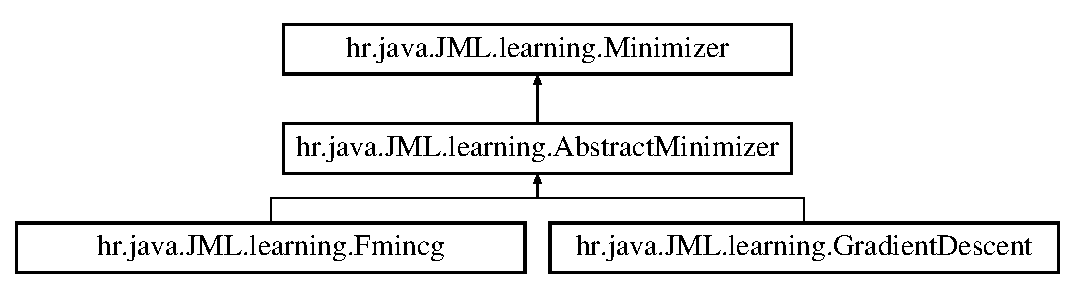
\includegraphics[height=3.000000cm]{classhr_1_1java_1_1_j_m_l_1_1learning_1_1_abstract_minimizer}
\end{center}
\end{figure}
\subsection*{Public Member Functions}
\begin{DoxyCompactItemize}
\item 
void \hyperlink{classhr_1_1java_1_1_j_m_l_1_1learning_1_1_abstract_minimizer_adbd6e7474e0ca526fb06f3abdcd2dff9}{add\+Iteration\+Completion\+Callback} (\hyperlink{interfacehr_1_1java_1_1_j_m_l_1_1learning_1_1_iteration_completion_listener}{Iteration\+Completion\+Listener} lst)
\end{DoxyCompactItemize}
\subsection*{Protected Member Functions}
\begin{DoxyCompactItemize}
\item 
final void \hyperlink{classhr_1_1java_1_1_j_m_l_1_1learning_1_1_abstract_minimizer_ad72fedd9f52c8c74b178bfac915b122f}{on\+Iteration\+Finished} (int iteration, double cost, Double\+Vector current\+Weights)
\end{DoxyCompactItemize}


\subsection{Detailed Description}
Abstract minimizer class that adds functionality that can be shared between many minimizers. Currently it has just a iteration completion callback facility, but can be later extended to share line searching code or other shared utilities.

\begin{DoxyAuthor}{Author}
thomas.\+jungblut 
\end{DoxyAuthor}


\subsection{Member Function Documentation}
\hypertarget{classhr_1_1java_1_1_j_m_l_1_1learning_1_1_abstract_minimizer_adbd6e7474e0ca526fb06f3abdcd2dff9}{\index{hr\+::java\+::\+J\+M\+L\+::learning\+::\+Abstract\+Minimizer@{hr\+::java\+::\+J\+M\+L\+::learning\+::\+Abstract\+Minimizer}!add\+Iteration\+Completion\+Callback@{add\+Iteration\+Completion\+Callback}}
\index{add\+Iteration\+Completion\+Callback@{add\+Iteration\+Completion\+Callback}!hr\+::java\+::\+J\+M\+L\+::learning\+::\+Abstract\+Minimizer@{hr\+::java\+::\+J\+M\+L\+::learning\+::\+Abstract\+Minimizer}}
\subsubsection[{add\+Iteration\+Completion\+Callback}]{\setlength{\rightskip}{0pt plus 5cm}void hr.\+java.\+J\+M\+L.\+learning.\+Abstract\+Minimizer.\+add\+Iteration\+Completion\+Callback (
\begin{DoxyParamCaption}
\item[{{\bf Iteration\+Completion\+Listener}}]{lst}
\end{DoxyParamCaption}
)}}\label{classhr_1_1java_1_1_j_m_l_1_1learning_1_1_abstract_minimizer_adbd6e7474e0ca526fb06f3abdcd2dff9}
Add a callback listener that triggers after a iteration.


\begin{DoxyParams}{Parameters}
{\em lst} & the iteration completion listener. \\
\hline
\end{DoxyParams}
\hypertarget{classhr_1_1java_1_1_j_m_l_1_1learning_1_1_abstract_minimizer_ad72fedd9f52c8c74b178bfac915b122f}{\index{hr\+::java\+::\+J\+M\+L\+::learning\+::\+Abstract\+Minimizer@{hr\+::java\+::\+J\+M\+L\+::learning\+::\+Abstract\+Minimizer}!on\+Iteration\+Finished@{on\+Iteration\+Finished}}
\index{on\+Iteration\+Finished@{on\+Iteration\+Finished}!hr\+::java\+::\+J\+M\+L\+::learning\+::\+Abstract\+Minimizer@{hr\+::java\+::\+J\+M\+L\+::learning\+::\+Abstract\+Minimizer}}
\subsubsection[{on\+Iteration\+Finished}]{\setlength{\rightskip}{0pt plus 5cm}final void hr.\+java.\+J\+M\+L.\+learning.\+Abstract\+Minimizer.\+on\+Iteration\+Finished (
\begin{DoxyParamCaption}
\item[{int}]{iteration, }
\item[{double}]{cost, }
\item[{Double\+Vector}]{current\+Weights}
\end{DoxyParamCaption}
)\hspace{0.3cm}{\ttfamily [protected]}}}\label{classhr_1_1java_1_1_j_m_l_1_1learning_1_1_abstract_minimizer_ad72fedd9f52c8c74b178bfac915b122f}
Callback method that should be called from an explicit subclass once an iteration was finished.


\begin{DoxyParams}{Parameters}
{\em iteration} & the number of the current iteration. \\
\hline
{\em cost} & the cost at the current iteration. \\
\hline
{\em current\+Weights} & the current optimal weights. \\
\hline
\end{DoxyParams}


The documentation for this class was generated from the following file\+:\begin{DoxyCompactItemize}
\item 
src/hr/java/\+J\+M\+L/learning/Abstract\+Minimizer.\+java\end{DoxyCompactItemize}

\hypertarget{classhr_1_1java_1_1_j_m_l_1_1activation_functions_1_1_activation_function}{\section{hr.\+java.\+J\+M\+L.\+activation\+Functions.\+Activation\+Function Class Reference}
\label{classhr_1_1java_1_1_j_m_l_1_1activation_functions_1_1_activation_function}\index{hr.\+java.\+J\+M\+L.\+activation\+Functions.\+Activation\+Function@{hr.\+java.\+J\+M\+L.\+activation\+Functions.\+Activation\+Function}}
}
Inheritance diagram for hr.\+java.\+J\+M\+L.\+activation\+Functions.\+Activation\+Function\+:\begin{figure}[H]
\begin{center}
\leavevmode
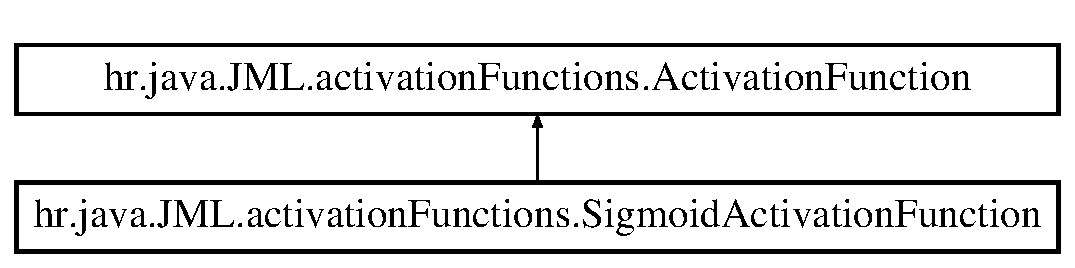
\includegraphics[height=2.000000cm]{classhr_1_1java_1_1_j_m_l_1_1activation_functions_1_1_activation_function}
\end{center}
\end{figure}
\subsection*{Public Member Functions}
\begin{DoxyCompactItemize}
\item 
\hypertarget{classhr_1_1java_1_1_j_m_l_1_1activation_functions_1_1_activation_function_a2bb203b04b008c4037748e9d9ff29719}{abstract double {\bfseries activation\+Function} (double input)}\label{classhr_1_1java_1_1_j_m_l_1_1activation_functions_1_1_activation_function_a2bb203b04b008c4037748e9d9ff29719}

\item 
\hypertarget{classhr_1_1java_1_1_j_m_l_1_1activation_functions_1_1_activation_function_a8c0c407aab3e7391d779498465f546f3}{abstract Double\+Vector {\bfseries activation\+Function} (Double\+Vector input)}\label{classhr_1_1java_1_1_j_m_l_1_1activation_functions_1_1_activation_function_a8c0c407aab3e7391d779498465f546f3}

\item 
\hypertarget{classhr_1_1java_1_1_j_m_l_1_1activation_functions_1_1_activation_function_a559bb68c2cf267adc19c4c08842194fd}{abstract Double\+Matrix {\bfseries activation\+Function} (Double\+Matrix input)}\label{classhr_1_1java_1_1_j_m_l_1_1activation_functions_1_1_activation_function_a559bb68c2cf267adc19c4c08842194fd}

\item 
\hypertarget{classhr_1_1java_1_1_j_m_l_1_1activation_functions_1_1_activation_function_afc4943d0df5f84bf26cc7245972f7942}{abstract Double\+Vector {\bfseries gradient} (Double\+Vector input)}\label{classhr_1_1java_1_1_j_m_l_1_1activation_functions_1_1_activation_function_afc4943d0df5f84bf26cc7245972f7942}

\item 
\hypertarget{classhr_1_1java_1_1_j_m_l_1_1activation_functions_1_1_activation_function_a688c4f6390aa1637b2cd35b4b6a14fe8}{abstract Double\+Matrix {\bfseries gradient} (Double\+Matrix input)}\label{classhr_1_1java_1_1_j_m_l_1_1activation_functions_1_1_activation_function_a688c4f6390aa1637b2cd35b4b6a14fe8}

\end{DoxyCompactItemize}


\subsection{Detailed Description}
\begin{DoxyAuthor}{Author}
Filip Habazin Computes the activation potentials and gradients of the input. 
\end{DoxyAuthor}


The documentation for this class was generated from the following file\+:\begin{DoxyCompactItemize}
\item 
src/hr/java/\+J\+M\+L/activation\+Functions/Activation\+Function.\+java\end{DoxyCompactItemize}

\hypertarget{interfacehr_1_1java_1_1_j_m_l_1_1cost_1_1_cost_function}{\section{hr.\+java.\+J\+M\+L.\+cost.\+Cost\+Function Interface Reference}
\label{interfacehr_1_1java_1_1_j_m_l_1_1cost_1_1_cost_function}\index{hr.\+java.\+J\+M\+L.\+cost.\+Cost\+Function@{hr.\+java.\+J\+M\+L.\+cost.\+Cost\+Function}}
}
\subsection*{Public Member Functions}
\begin{DoxyCompactItemize}
\item 
\hyperlink{classhr_1_1java_1_1_j_m_l_1_1cost_1_1_cost_gradient_tuple}{Cost\+Gradient\+Tuple} \hyperlink{interfacehr_1_1java_1_1_j_m_l_1_1cost_1_1_cost_function_aa63d4185cba8b1f5887093ff9ba7db9a}{evaluate\+Cost} (Double\+Vector input)
\end{DoxyCompactItemize}


\subsection{Detailed Description}
Cost function interface to be implemented when using with a optimizer like conjugate gradient for example.

\begin{DoxyAuthor}{Author}
thomas.\+jungblut 
\end{DoxyAuthor}


\subsection{Member Function Documentation}
\hypertarget{interfacehr_1_1java_1_1_j_m_l_1_1cost_1_1_cost_function_aa63d4185cba8b1f5887093ff9ba7db9a}{\index{hr\+::java\+::\+J\+M\+L\+::cost\+::\+Cost\+Function@{hr\+::java\+::\+J\+M\+L\+::cost\+::\+Cost\+Function}!evaluate\+Cost@{evaluate\+Cost}}
\index{evaluate\+Cost@{evaluate\+Cost}!hr\+::java\+::\+J\+M\+L\+::cost\+::\+Cost\+Function@{hr\+::java\+::\+J\+M\+L\+::cost\+::\+Cost\+Function}}
\subsubsection[{evaluate\+Cost}]{\setlength{\rightskip}{0pt plus 5cm}{\bf Cost\+Gradient\+Tuple} hr.\+java.\+J\+M\+L.\+cost.\+Cost\+Function.\+evaluate\+Cost (
\begin{DoxyParamCaption}
\item[{Double\+Vector}]{input}
\end{DoxyParamCaption}
)}}\label{interfacehr_1_1java_1_1_j_m_l_1_1cost_1_1_cost_function_aa63d4185cba8b1f5887093ff9ba7db9a}
Evaluation for the cost function to retrieve cost and gradient.


\begin{DoxyParams}{Parameters}
{\em input} & a given input vector \\
\hline
\end{DoxyParams}
\begin{DoxyReturn}{Returns}
a tuple consists of J (cost) and a vector X which is the gradient of the input. 
\end{DoxyReturn}


The documentation for this interface was generated from the following file\+:\begin{DoxyCompactItemize}
\item 
src/hr/java/\+J\+M\+L/cost/Cost\+Function.\+java\end{DoxyCompactItemize}

\hypertarget{classhr_1_1java_1_1_j_m_l_1_1cost_1_1_cost_gradient_tuple}{\section{hr.\+java.\+J\+M\+L.\+cost.\+Cost\+Gradient\+Tuple Class Reference}
\label{classhr_1_1java_1_1_j_m_l_1_1cost_1_1_cost_gradient_tuple}\index{hr.\+java.\+J\+M\+L.\+cost.\+Cost\+Gradient\+Tuple@{hr.\+java.\+J\+M\+L.\+cost.\+Cost\+Gradient\+Tuple}}
}
\subsection*{Public Member Functions}
\begin{DoxyCompactItemize}
\item 
\hypertarget{classhr_1_1java_1_1_j_m_l_1_1cost_1_1_cost_gradient_tuple_a06970ea1ada93ebac1abe6ebbde8dfd0}{{\bfseries Cost\+Gradient\+Tuple} (double cost, Double\+Vector gradient)}\label{classhr_1_1java_1_1_j_m_l_1_1cost_1_1_cost_gradient_tuple_a06970ea1ada93ebac1abe6ebbde8dfd0}

\item 
\hypertarget{classhr_1_1java_1_1_j_m_l_1_1cost_1_1_cost_gradient_tuple_aa6342f2d6d3573cbb838b1f49766d18e}{double {\bfseries get\+Cost} ()}\label{classhr_1_1java_1_1_j_m_l_1_1cost_1_1_cost_gradient_tuple_aa6342f2d6d3573cbb838b1f49766d18e}

\item 
\hypertarget{classhr_1_1java_1_1_j_m_l_1_1cost_1_1_cost_gradient_tuple_a22954db9f670eb20c41caaf208d4f627}{Double\+Vector {\bfseries get\+Gradient} ()}\label{classhr_1_1java_1_1_j_m_l_1_1cost_1_1_cost_gradient_tuple_a22954db9f670eb20c41caaf208d4f627}

\end{DoxyCompactItemize}


\subsection{Detailed Description}
More readable variant of the before used Tuple$<$$>$ in \hyperlink{interfacehr_1_1java_1_1_j_m_l_1_1cost_1_1_cost_function}{Cost\+Function}.

\begin{DoxyAuthor}{Author}
thomas.\+jungblut 
\end{DoxyAuthor}


The documentation for this class was generated from the following file\+:\begin{DoxyCompactItemize}
\item 
src/hr/java/\+J\+M\+L/cost/Cost\+Gradient\+Tuple.\+java\end{DoxyCompactItemize}

\hypertarget{classhr_1_1java_1_1_j_m_l_1_1util_1_1_dense_matrix_folder}{\section{hr.\+java.\+J\+M\+L.\+util.\+Dense\+Matrix\+Folder Class Reference}
\label{classhr_1_1java_1_1_j_m_l_1_1util_1_1_dense_matrix_folder}\index{hr.\+java.\+J\+M\+L.\+util.\+Dense\+Matrix\+Folder@{hr.\+java.\+J\+M\+L.\+util.\+Dense\+Matrix\+Folder}}
}
\subsection*{Static Public Member Functions}
\begin{DoxyCompactItemize}
\item 
static Double\+Vector \hyperlink{classhr_1_1java_1_1_j_m_l_1_1util_1_1_dense_matrix_folder_a322a9d5a5af15ffeca0a11e7772761ab}{fold\+Matrices} (Double\+Matrix...\+matrices)
\item 
static Double\+Matrix\mbox{[}$\,$\mbox{]} \hyperlink{classhr_1_1java_1_1_j_m_l_1_1util_1_1_dense_matrix_folder_a0d9c5a40c979367df898348c4781b1eb}{unfold\+Matrices} (Double\+Vector vector, int\mbox{[}$\,$\mbox{]}\mbox{[}$\,$\mbox{]} size\+Array)
\item 
static Double\+Matrix \hyperlink{classhr_1_1java_1_1_j_m_l_1_1util_1_1_dense_matrix_folder_ad64e17bc9f959157f5e857be642b00a5}{unfold\+Matrix} (Double\+Vector vector, int rows, int cols)
\item 
static Double\+Vector \hyperlink{classhr_1_1java_1_1_j_m_l_1_1util_1_1_dense_matrix_folder_abf332d6e1120572283da3a7c49166095}{fold\+Matrix} (Double\+Matrix mat)
\end{DoxyCompactItemize}


\subsection{Member Function Documentation}
\hypertarget{classhr_1_1java_1_1_j_m_l_1_1util_1_1_dense_matrix_folder_a322a9d5a5af15ffeca0a11e7772761ab}{\index{hr\+::java\+::\+J\+M\+L\+::util\+::\+Dense\+Matrix\+Folder@{hr\+::java\+::\+J\+M\+L\+::util\+::\+Dense\+Matrix\+Folder}!fold\+Matrices@{fold\+Matrices}}
\index{fold\+Matrices@{fold\+Matrices}!hr\+::java\+::\+J\+M\+L\+::util\+::\+Dense\+Matrix\+Folder@{hr\+::java\+::\+J\+M\+L\+::util\+::\+Dense\+Matrix\+Folder}}
\subsubsection[{fold\+Matrices}]{\setlength{\rightskip}{0pt plus 5cm}static Double\+Vector hr.\+java.\+J\+M\+L.\+util.\+Dense\+Matrix\+Folder.\+fold\+Matrices (
\begin{DoxyParamCaption}
\item[{Double\+Matrix...}]{matrices}
\end{DoxyParamCaption}
)\hspace{0.3cm}{\ttfamily [static]}}}\label{classhr_1_1java_1_1_j_m_l_1_1util_1_1_dense_matrix_folder_a322a9d5a5af15ffeca0a11e7772761ab}
Folds the given matrices column-\/wise into a single vector. \hypertarget{classhr_1_1java_1_1_j_m_l_1_1util_1_1_dense_matrix_folder_abf332d6e1120572283da3a7c49166095}{\index{hr\+::java\+::\+J\+M\+L\+::util\+::\+Dense\+Matrix\+Folder@{hr\+::java\+::\+J\+M\+L\+::util\+::\+Dense\+Matrix\+Folder}!fold\+Matrix@{fold\+Matrix}}
\index{fold\+Matrix@{fold\+Matrix}!hr\+::java\+::\+J\+M\+L\+::util\+::\+Dense\+Matrix\+Folder@{hr\+::java\+::\+J\+M\+L\+::util\+::\+Dense\+Matrix\+Folder}}
\subsubsection[{fold\+Matrix}]{\setlength{\rightskip}{0pt plus 5cm}static Double\+Vector hr.\+java.\+J\+M\+L.\+util.\+Dense\+Matrix\+Folder.\+fold\+Matrix (
\begin{DoxyParamCaption}
\item[{Double\+Matrix}]{mat}
\end{DoxyParamCaption}
)\hspace{0.3cm}{\ttfamily [static]}}}\label{classhr_1_1java_1_1_j_m_l_1_1util_1_1_dense_matrix_folder_abf332d6e1120572283da3a7c49166095}
Folds a single matrix into a single vector by rows. \hypertarget{classhr_1_1java_1_1_j_m_l_1_1util_1_1_dense_matrix_folder_a0d9c5a40c979367df898348c4781b1eb}{\index{hr\+::java\+::\+J\+M\+L\+::util\+::\+Dense\+Matrix\+Folder@{hr\+::java\+::\+J\+M\+L\+::util\+::\+Dense\+Matrix\+Folder}!unfold\+Matrices@{unfold\+Matrices}}
\index{unfold\+Matrices@{unfold\+Matrices}!hr\+::java\+::\+J\+M\+L\+::util\+::\+Dense\+Matrix\+Folder@{hr\+::java\+::\+J\+M\+L\+::util\+::\+Dense\+Matrix\+Folder}}
\subsubsection[{unfold\+Matrices}]{\setlength{\rightskip}{0pt plus 5cm}static Double\+Matrix \mbox{[}$\,$\mbox{]} hr.\+java.\+J\+M\+L.\+util.\+Dense\+Matrix\+Folder.\+unfold\+Matrices (
\begin{DoxyParamCaption}
\item[{Double\+Vector}]{vector, }
\item[{int}]{size\+Array\mbox{[}$\,$\mbox{]}\mbox{[}$\,$\mbox{]}}
\end{DoxyParamCaption}
)\hspace{0.3cm}{\ttfamily [static]}}}\label{classhr_1_1java_1_1_j_m_l_1_1util_1_1_dense_matrix_folder_a0d9c5a40c979367df898348c4781b1eb}
Unfolds a vector into matrices by the rules defined in the size\+Array. The size\+Array must have following format\+: in each row the row and column count must be provided.~\newline
 Example\+: size\+Array = \{\{2,3\},\{3,2\}\} will unfold into matrix 0 with 2 rows and 3 columns and matrix 1 with 3 rows and 2 columns. \hypertarget{classhr_1_1java_1_1_j_m_l_1_1util_1_1_dense_matrix_folder_ad64e17bc9f959157f5e857be642b00a5}{\index{hr\+::java\+::\+J\+M\+L\+::util\+::\+Dense\+Matrix\+Folder@{hr\+::java\+::\+J\+M\+L\+::util\+::\+Dense\+Matrix\+Folder}!unfold\+Matrix@{unfold\+Matrix}}
\index{unfold\+Matrix@{unfold\+Matrix}!hr\+::java\+::\+J\+M\+L\+::util\+::\+Dense\+Matrix\+Folder@{hr\+::java\+::\+J\+M\+L\+::util\+::\+Dense\+Matrix\+Folder}}
\subsubsection[{unfold\+Matrix}]{\setlength{\rightskip}{0pt plus 5cm}static Double\+Matrix hr.\+java.\+J\+M\+L.\+util.\+Dense\+Matrix\+Folder.\+unfold\+Matrix (
\begin{DoxyParamCaption}
\item[{Double\+Vector}]{vector, }
\item[{int}]{rows, }
\item[{int}]{cols}
\end{DoxyParamCaption}
)\hspace{0.3cm}{\ttfamily [static]}}}\label{classhr_1_1java_1_1_j_m_l_1_1util_1_1_dense_matrix_folder_ad64e17bc9f959157f5e857be642b00a5}
Unfolds a single vector into a single matrix by rows.


\begin{DoxyParams}{Parameters}
{\em vector} & the vector to split. \\
\hline
{\em rows} & the number of rows the target matrix needs to have. \\
\hline
{\em cols} & the number of columns the target matrix needs to have. \\
\hline
\end{DoxyParams}
\begin{DoxyReturn}{Returns}
a matrix with the contents of the vector, row split. 
\end{DoxyReturn}


The documentation for this class was generated from the following file\+:\begin{DoxyCompactItemize}
\item 
src/hr/java/\+J\+M\+L/util/Dense\+Matrix\+Folder.\+java\end{DoxyCompactItemize}

\hypertarget{classhr_1_1java_1_1_j_m_l_1_1neural_1_1_double_input_layer}{\section{hr.\+java.\+J\+M\+L.\+neural.\+Double\+Input\+Layer Class Reference}
\label{classhr_1_1java_1_1_j_m_l_1_1neural_1_1_double_input_layer}\index{hr.\+java.\+J\+M\+L.\+neural.\+Double\+Input\+Layer@{hr.\+java.\+J\+M\+L.\+neural.\+Double\+Input\+Layer}}
}
Inheritance diagram for hr.\+java.\+J\+M\+L.\+neural.\+Double\+Input\+Layer\+:\begin{figure}[H]
\begin{center}
\leavevmode
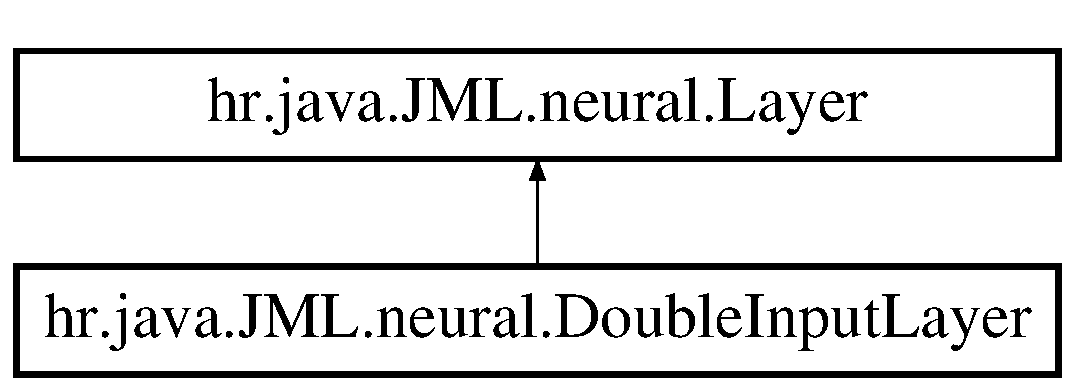
\includegraphics[height=2.000000cm]{classhr_1_1java_1_1_j_m_l_1_1neural_1_1_double_input_layer}
\end{center}
\end{figure}
\subsection*{Public Member Functions}
\begin{DoxyCompactItemize}
\item 
\hypertarget{classhr_1_1java_1_1_j_m_l_1_1neural_1_1_double_input_layer_a01f1be70667315d831804a9ca7ee0169}{{\bfseries Double\+Input\+Layer} (int input\+Size)}\label{classhr_1_1java_1_1_j_m_l_1_1neural_1_1_double_input_layer_a01f1be70667315d831804a9ca7ee0169}

\item 
\hypertarget{classhr_1_1java_1_1_j_m_l_1_1neural_1_1_double_input_layer_a559a54af247c046ddf45fb7e6945313c}{Double\+Vector {\bfseries calculate\+Output} (Double\+Vector input)}\label{classhr_1_1java_1_1_j_m_l_1_1neural_1_1_double_input_layer_a559a54af247c046ddf45fb7e6945313c}

\end{DoxyCompactItemize}
\subsection*{Additional Inherited Members}


The documentation for this class was generated from the following file\+:\begin{DoxyCompactItemize}
\item 
src/hr/java/\+J\+M\+L/neural/Double\+Input\+Layer.\+java\end{DoxyCompactItemize}

\hypertarget{classhr_1_1java_1_1_j_m_l_1_1normalization_1_1_feature_normalizer}{\section{hr.\+java.\+J\+M\+L.\+normalization.\+Feature\+Normalizer Class Reference}
\label{classhr_1_1java_1_1_j_m_l_1_1normalization_1_1_feature_normalizer}\index{hr.\+java.\+J\+M\+L.\+normalization.\+Feature\+Normalizer@{hr.\+java.\+J\+M\+L.\+normalization.\+Feature\+Normalizer}}
}
\subsection*{Static Public Member Functions}
\begin{DoxyCompactItemize}
\item 
\hypertarget{classhr_1_1java_1_1_j_m_l_1_1normalization_1_1_feature_normalizer_ad0dc45ee779d52a913fa23de1a9129fc}{static double\mbox{[}$\,$\mbox{]} {\bfseries normalizer} (double\mbox{[}$\,$\mbox{]} features)}\label{classhr_1_1java_1_1_j_m_l_1_1normalization_1_1_feature_normalizer_ad0dc45ee779d52a913fa23de1a9129fc}

\end{DoxyCompactItemize}


The documentation for this class was generated from the following file\+:\begin{DoxyCompactItemize}
\item 
src/hr/java/\+J\+M\+L/normalization/Feature\+Normalizer.\+java\end{DoxyCompactItemize}

\hypertarget{classhr_1_1java_1_1_j_m_l_1_1learning_1_1_fmincg}{\section{hr.\+java.\+J\+M\+L.\+learning.\+Fmincg Class Reference}
\label{classhr_1_1java_1_1_j_m_l_1_1learning_1_1_fmincg}\index{hr.\+java.\+J\+M\+L.\+learning.\+Fmincg@{hr.\+java.\+J\+M\+L.\+learning.\+Fmincg}}
}
Inheritance diagram for hr.\+java.\+J\+M\+L.\+learning.\+Fmincg\+:\begin{figure}[H]
\begin{center}
\leavevmode
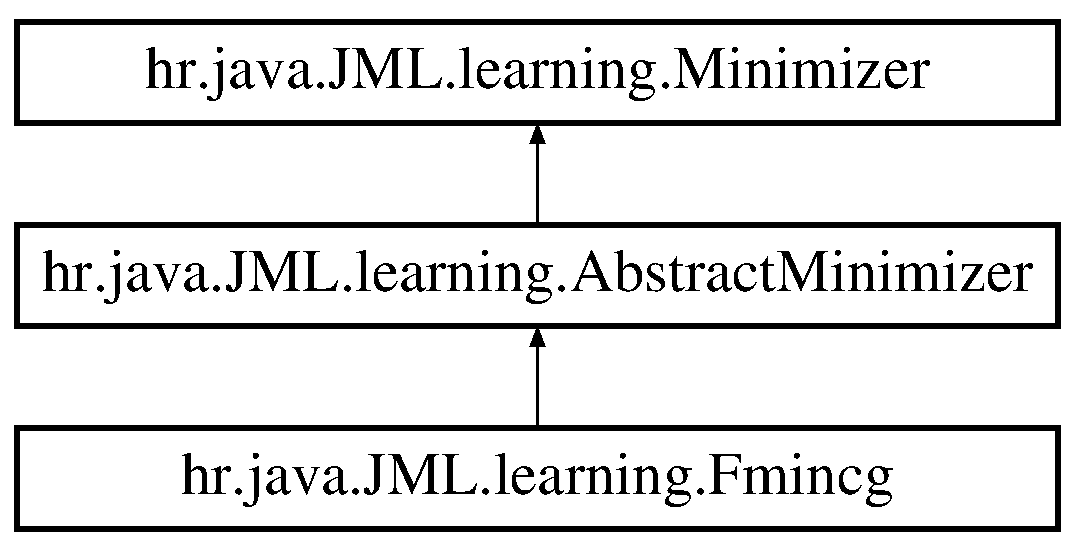
\includegraphics[height=3.000000cm]{classhr_1_1java_1_1_j_m_l_1_1learning_1_1_fmincg}
\end{center}
\end{figure}
\subsection*{Public Member Functions}
\begin{DoxyCompactItemize}
\item 
final Double\+Vector \hyperlink{classhr_1_1java_1_1_j_m_l_1_1learning_1_1_fmincg_a91e1dfdbc2222e1844a3c6d079a7e3e7}{minimize} (\hyperlink{interfacehr_1_1java_1_1_j_m_l_1_1cost_1_1_cost_function}{Cost\+Function} f, Double\+Vector theta, int length, boolean verbose)
\end{DoxyCompactItemize}
\subsection*{Static Public Member Functions}
\begin{DoxyCompactItemize}
\item 
static Double\+Vector \hyperlink{classhr_1_1java_1_1_j_m_l_1_1learning_1_1_fmincg_a214ab4364ba5cba6fdf1bcebd6d74be5}{minimize\+Function} (\hyperlink{interfacehr_1_1java_1_1_j_m_l_1_1cost_1_1_cost_function}{Cost\+Function} f, Double\+Vector theta, int max\+Iterations, boolean verbose)
\end{DoxyCompactItemize}
\subsection*{Static Public Attributes}
\begin{DoxyCompactItemize}
\item 
\hypertarget{classhr_1_1java_1_1_j_m_l_1_1learning_1_1_fmincg_a2a668ac99dd7384c2328358bdecfc7fe}{static double {\bfseries E\+X\+T} = 3.\+0}\label{classhr_1_1java_1_1_j_m_l_1_1learning_1_1_fmincg_a2a668ac99dd7384c2328358bdecfc7fe}

\end{DoxyCompactItemize}
\subsection*{Additional Inherited Members}


\subsection{Detailed Description}
Minimize a continuous differentialble multivariate function. Starting point ~\newline
 is given by \char`\"{}\+X\char`\"{} (D by 1), and the function named in the string \char`\"{}f\char`\"{}, must~\newline
 return a function value and a vector of partial derivatives. The Polack-\/~\newline
 Ribiere flavour of conjugate gradients is used to compute search directions,~\newline
 and a line search using quadratic and cubic polynomial approximations and the~\newline
 Wolfe-\/\+Powell stopping criteria is used together with the slope ratio method~\newline
 for guessing initial step sizes. Additionally a bunch of checks are made to~\newline
 make sure that exploration is taking place and that extrapolation will not~\newline
 be unboundedly large. The \char`\"{}length\char`\"{} gives the length of the run\+: if it is~\newline
 positive, it gives the maximum number of line searches, if negative its~\newline
 absolute gives the maximum allowed number of function evaluations. You can~\newline
 (optionally) give \char`\"{}length\char`\"{} a second component, which will indicate the~\newline
 reduction in function value to be expected in the first line-\/search (defaults~\newline
 to 1.\+0). The function returns when either its length is up, or if no further~\newline
 progress can be made (ie, we are at a minimum, or so close that due to~\newline
 numerical problems, we cannot get any closer). If the function terminates~\newline
 within a few iterations, it could be an indication that the function value~\newline
 and derivatives are not consistent (ie, there may be a bug in the~\newline
 implementation of your \char`\"{}f\char`\"{} function). The function returns the found~\newline
 solution \char`\"{}\+X\char`\"{}, a vector of function values \char`\"{}f\+X\char`\"{} indicating the progress made~\newline
 and \char`\"{}i\char`\"{} the number of iterations (line searches or function evaluations,~\newline
 depending on the sign of \char`\"{}length\char`\"{}) used.~\newline
 ~\newline
 Usage\+: \mbox{[}X, f\+X, i\mbox{]} = fmincg(f, X, options, P1, P2, P3, P4, P5)~\newline
 ~\newline
 See also\+: checkgrad ~\newline
 ~\newline
 Copyright (C) 2001 and 2002 by Carl Edward Rasmussen. Date 2002-\/02-\/13~\newline
 ~\newline
 ~\newline
 (C) Copyright 1999, 2000 \& 2001, Carl Edward Rasmussen ~\newline
 Permission is granted for anyone to copy, use, or modify these~\newline
 programs and accompanying documents for purposes of research or~\newline
 education, provided this copyright notice is retained, and note is~\newline
 made of any changes that have been made.~\newline
 ~\newline
 These programs and documents are distributed without any warranty,~\newline
 express or implied. As the programs were written for research~\newline
 purposes only, they have not been tested to the degree that would be~\newline
 advisable in any important application. All use of these programs is~\newline
 entirely at the user's own risk.~\newline
 ~\newline
 \mbox{[}ml-\/class\mbox{]} Changes Made\+:~\newline
 1) Function name and argument specifications~\newline
 2) Output display~\newline
 ~\newline
 \mbox{[}tjungblut\mbox{]} Changes Made\+: ~\newline
 1) translated from octave to java~\newline
 2) added an interface to exchange minimizers more easily ~\newline
 3) in preparation for the c++ translation, I removed unused fields~\newline
 B\+T\+W \char`\"{}fmincg\char`\"{} stands for Function minimize nonlinear conjugate gradient 

\subsection{Member Function Documentation}
\hypertarget{classhr_1_1java_1_1_j_m_l_1_1learning_1_1_fmincg_a91e1dfdbc2222e1844a3c6d079a7e3e7}{\index{hr\+::java\+::\+J\+M\+L\+::learning\+::\+Fmincg@{hr\+::java\+::\+J\+M\+L\+::learning\+::\+Fmincg}!minimize@{minimize}}
\index{minimize@{minimize}!hr\+::java\+::\+J\+M\+L\+::learning\+::\+Fmincg@{hr\+::java\+::\+J\+M\+L\+::learning\+::\+Fmincg}}
\subsubsection[{minimize}]{\setlength{\rightskip}{0pt plus 5cm}final Double\+Vector hr.\+java.\+J\+M\+L.\+learning.\+Fmincg.\+minimize (
\begin{DoxyParamCaption}
\item[{{\bf Cost\+Function}}]{f, }
\item[{Double\+Vector}]{theta, }
\item[{int}]{max\+Iterations, }
\item[{boolean}]{verbose}
\end{DoxyParamCaption}
)}}\label{classhr_1_1java_1_1_j_m_l_1_1learning_1_1_fmincg_a91e1dfdbc2222e1844a3c6d079a7e3e7}
Minimizes the given costfunction with the starting parameter theta.


\begin{DoxyParams}{Parameters}
{\em f} & the costfunction to minimize. \\
\hline
{\em theta} & the starting parameters. \\
\hline
{\em max\+Iterations} & the number of iterations to do. \\
\hline
{\em verbose} & if T\+R\+U\+E it will print progress. \\
\hline
\end{DoxyParams}
\begin{DoxyReturn}{Returns}
the optimized theta parameters. 
\end{DoxyReturn}


Implements \hyperlink{interfacehr_1_1java_1_1_j_m_l_1_1learning_1_1_minimizer_a4b640a5d2cc5293ccc47736a798c6ab7}{hr.\+java.\+J\+M\+L.\+learning.\+Minimizer}.

\hypertarget{classhr_1_1java_1_1_j_m_l_1_1learning_1_1_fmincg_a214ab4364ba5cba6fdf1bcebd6d74be5}{\index{hr\+::java\+::\+J\+M\+L\+::learning\+::\+Fmincg@{hr\+::java\+::\+J\+M\+L\+::learning\+::\+Fmincg}!minimize\+Function@{minimize\+Function}}
\index{minimize\+Function@{minimize\+Function}!hr\+::java\+::\+J\+M\+L\+::learning\+::\+Fmincg@{hr\+::java\+::\+J\+M\+L\+::learning\+::\+Fmincg}}
\subsubsection[{minimize\+Function}]{\setlength{\rightskip}{0pt plus 5cm}static Double\+Vector hr.\+java.\+J\+M\+L.\+learning.\+Fmincg.\+minimize\+Function (
\begin{DoxyParamCaption}
\item[{{\bf Cost\+Function}}]{f, }
\item[{Double\+Vector}]{theta, }
\item[{int}]{max\+Iterations, }
\item[{boolean}]{verbose}
\end{DoxyParamCaption}
)\hspace{0.3cm}{\ttfamily [static]}}}\label{classhr_1_1java_1_1_j_m_l_1_1learning_1_1_fmincg_a214ab4364ba5cba6fdf1bcebd6d74be5}
Minimizes the given Cost\+Function with Nonlinear conjugate gradient method. ~\newline
 It uses the Polack-\/\+Ribiere (P\+R) to calculate the conjugate direction. See ~\newline
 \hyperlink{}{http\+://en.\+wikipedia.\+org/wiki/\+Nonlinear\+\_\+conjugate\+\_\+gradient\+\_\+method} ~\newline
 for more information.


\begin{DoxyParams}{Parameters}
{\em f} & the cost function to minimize. \\
\hline
{\em theta} & the input vector, also called starting point \\
\hline
{\em max\+Iterations} & the number of iterations to make \\
\hline
{\em verbose} & output the progress to S\+T\+D\+O\+U\+T \\
\hline
\end{DoxyParams}
\begin{DoxyReturn}{Returns}
a vector containing the optimized input 
\end{DoxyReturn}


The documentation for this class was generated from the following file\+:\begin{DoxyCompactItemize}
\item 
src/hr/java/\+J\+M\+L/learning/Fmincg.\+java\end{DoxyCompactItemize}

\hypertarget{classhr_1_1java_1_1_j_m_l_1_1learning_1_1_gradient_descent}{\section{hr.\+java.\+J\+M\+L.\+learning.\+Gradient\+Descent Class Reference}
\label{classhr_1_1java_1_1_j_m_l_1_1learning_1_1_gradient_descent}\index{hr.\+java.\+J\+M\+L.\+learning.\+Gradient\+Descent@{hr.\+java.\+J\+M\+L.\+learning.\+Gradient\+Descent}}
}
Inheritance diagram for hr.\+java.\+J\+M\+L.\+learning.\+Gradient\+Descent\+:\begin{figure}[H]
\begin{center}
\leavevmode
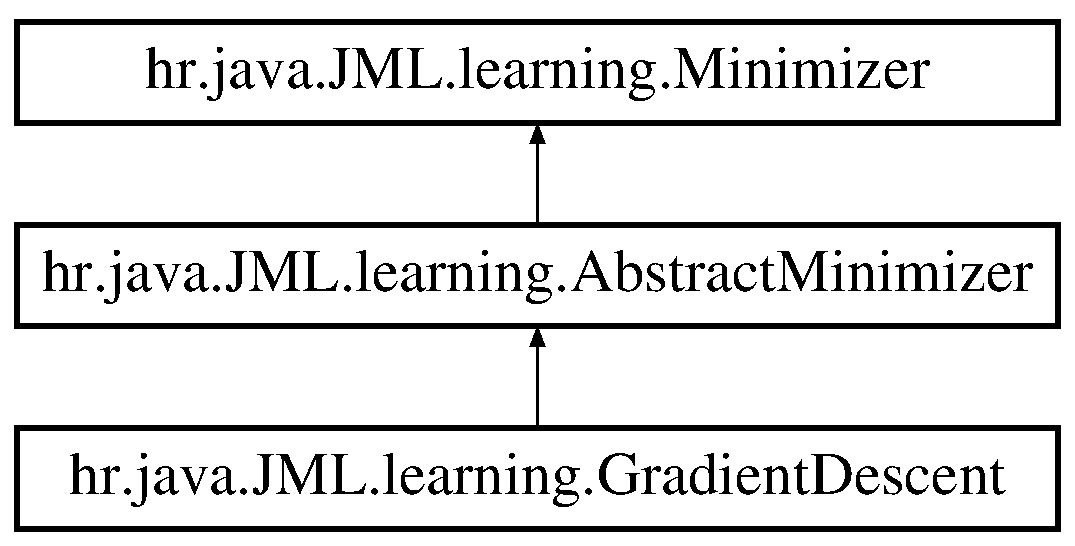
\includegraphics[height=3.000000cm]{classhr_1_1java_1_1_j_m_l_1_1learning_1_1_gradient_descent}
\end{center}
\end{figure}
\subsection*{Classes}
\begin{DoxyCompactItemize}
\item 
class {\bfseries Gradient\+Descent\+Builder}
\end{DoxyCompactItemize}
\subsection*{Public Member Functions}
\begin{DoxyCompactItemize}
\item 
\hyperlink{classhr_1_1java_1_1_j_m_l_1_1learning_1_1_gradient_descent_aa32d3a402cf616e329e99edb77fc158b}{Gradient\+Descent} (double alpha, double limit)
\item 
\hypertarget{classhr_1_1java_1_1_j_m_l_1_1learning_1_1_gradient_descent_a86328bc9a0e726c3cb170c9ff7f2f5d2}{final Double\+Vector {\bfseries minimize} (\hyperlink{interfacehr_1_1java_1_1_j_m_l_1_1cost_1_1_cost_function}{Cost\+Function} f, Double\+Vector p\+Input, final int max\+Iterations, boolean verbose)}\label{classhr_1_1java_1_1_j_m_l_1_1learning_1_1_gradient_descent_a86328bc9a0e726c3cb170c9ff7f2f5d2}

\end{DoxyCompactItemize}
\subsection*{Static Public Member Functions}
\begin{DoxyCompactItemize}
\item 
static Double\+Vector \hyperlink{classhr_1_1java_1_1_j_m_l_1_1learning_1_1_gradient_descent_a3506167dfc8e64ff2104c63be5ec58f7}{minimize\+Function} (\hyperlink{interfacehr_1_1java_1_1_j_m_l_1_1cost_1_1_cost_function}{Cost\+Function} f, Double\+Vector p\+Input, double alpha, double limit, int length, final boolean verbose)
\end{DoxyCompactItemize}
\subsection*{Additional Inherited Members}


\subsection{Detailed Description}
Gradient descent implementation with some neat features like momentum, divergence detection, delta breaks and bold driver and scheduled annealing adaptive learning rates. For more sophisticated configuration use the \hyperlink{}{Gradient\+Descent\+Builder}.

\begin{DoxyAuthor}{Author}
thomas.\+jungblut 
\end{DoxyAuthor}


\subsection{Constructor \& Destructor Documentation}
\hypertarget{classhr_1_1java_1_1_j_m_l_1_1learning_1_1_gradient_descent_aa32d3a402cf616e329e99edb77fc158b}{\index{hr\+::java\+::\+J\+M\+L\+::learning\+::\+Gradient\+Descent@{hr\+::java\+::\+J\+M\+L\+::learning\+::\+Gradient\+Descent}!Gradient\+Descent@{Gradient\+Descent}}
\index{Gradient\+Descent@{Gradient\+Descent}!hr\+::java\+::\+J\+M\+L\+::learning\+::\+Gradient\+Descent@{hr\+::java\+::\+J\+M\+L\+::learning\+::\+Gradient\+Descent}}
\subsubsection[{Gradient\+Descent}]{\setlength{\rightskip}{0pt plus 5cm}hr.\+java.\+J\+M\+L.\+learning.\+Gradient\+Descent.\+Gradient\+Descent (
\begin{DoxyParamCaption}
\item[{double}]{alpha, }
\item[{double}]{limit}
\end{DoxyParamCaption}
)}}\label{classhr_1_1java_1_1_j_m_l_1_1learning_1_1_gradient_descent_aa32d3a402cf616e329e99edb77fc158b}

\begin{DoxyParams}{Parameters}
{\em alpha} & the learning rate. \\
\hline
{\em limit} & the delta in cost to archieve to break the iterations. \\
\hline
\end{DoxyParams}


\subsection{Member Function Documentation}
\hypertarget{classhr_1_1java_1_1_j_m_l_1_1learning_1_1_gradient_descent_a3506167dfc8e64ff2104c63be5ec58f7}{\index{hr\+::java\+::\+J\+M\+L\+::learning\+::\+Gradient\+Descent@{hr\+::java\+::\+J\+M\+L\+::learning\+::\+Gradient\+Descent}!minimize\+Function@{minimize\+Function}}
\index{minimize\+Function@{minimize\+Function}!hr\+::java\+::\+J\+M\+L\+::learning\+::\+Gradient\+Descent@{hr\+::java\+::\+J\+M\+L\+::learning\+::\+Gradient\+Descent}}
\subsubsection[{minimize\+Function}]{\setlength{\rightskip}{0pt plus 5cm}static Double\+Vector hr.\+java.\+J\+M\+L.\+learning.\+Gradient\+Descent.\+minimize\+Function (
\begin{DoxyParamCaption}
\item[{{\bf Cost\+Function}}]{f, }
\item[{Double\+Vector}]{p\+Input, }
\item[{double}]{alpha, }
\item[{double}]{limit, }
\item[{int}]{length, }
\item[{final boolean}]{verbose}
\end{DoxyParamCaption}
)\hspace{0.3cm}{\ttfamily [static]}}}\label{classhr_1_1java_1_1_j_m_l_1_1learning_1_1_gradient_descent_a3506167dfc8e64ff2104c63be5ec58f7}
Minimize a given cost function f with the initial parameters p\+Input (also called theta) with a learning rate alpha and a fixed number of iterations. The loop can break earlier if costs converge below the limit. If the same cost was archieved three times in a row, it will also break the iterations.


\begin{DoxyParams}{Parameters}
{\em f} & the function to minimize. \\
\hline
{\em p\+Input} & the starting parameters. \\
\hline
{\em alpha} & the learning rate. \\
\hline
{\em limit} & the cost to archieve to break the iterations. \\
\hline
{\em length} & the number of iterations. \\
\hline
{\em verbose} & if true prints progress to S\+T\+D\+O\+U\+T. \\
\hline
\end{DoxyParams}
\begin{DoxyReturn}{Returns}
the learned minimal parameters. 
\end{DoxyReturn}


The documentation for this class was generated from the following file\+:\begin{DoxyCompactItemize}
\item 
src/hr/java/\+J\+M\+L/learning/Gradient\+Descent.\+java\end{DoxyCompactItemize}

\hypertarget{classhr_1_1java_1_1_j_m_l_1_1neural_1_1_hidden_layer}{\section{hr.\+java.\+J\+M\+L.\+neural.\+Hidden\+Layer Class Reference}
\label{classhr_1_1java_1_1_j_m_l_1_1neural_1_1_hidden_layer}\index{hr.\+java.\+J\+M\+L.\+neural.\+Hidden\+Layer@{hr.\+java.\+J\+M\+L.\+neural.\+Hidden\+Layer}}
}
Inheritance diagram for hr.\+java.\+J\+M\+L.\+neural.\+Hidden\+Layer\+:\begin{figure}[H]
\begin{center}
\leavevmode
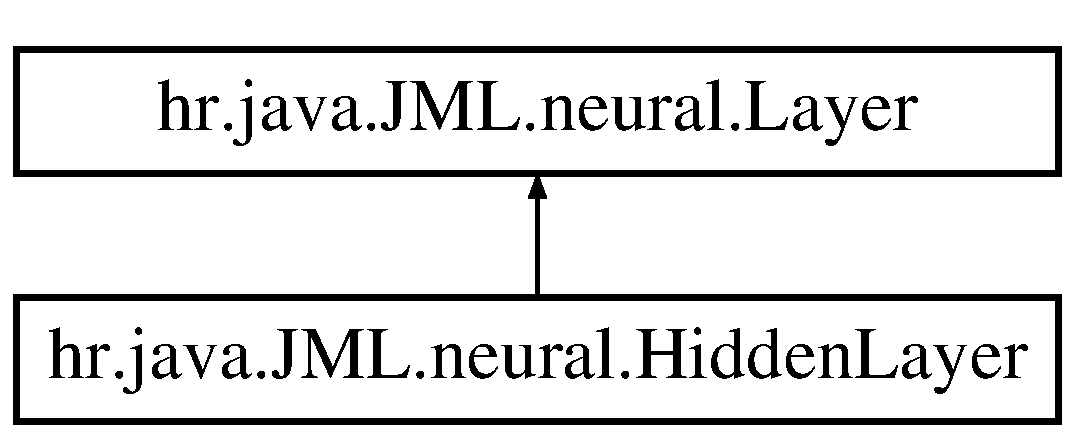
\includegraphics[height=2.000000cm]{classhr_1_1java_1_1_j_m_l_1_1neural_1_1_hidden_layer}
\end{center}
\end{figure}
\subsection*{Public Member Functions}
\begin{DoxyCompactItemize}
\item 
\hypertarget{classhr_1_1java_1_1_j_m_l_1_1neural_1_1_hidden_layer_a06bec6318a3df6d8875456a929b6c7be}{{\bfseries Hidden\+Layer} (int size, \hyperlink{classhr_1_1java_1_1_j_m_l_1_1neural_1_1_layer}{Layer} prev, \hyperlink{classhr_1_1java_1_1_j_m_l_1_1activation_functions_1_1_activation_function}{Activation\+Function} af)}\label{classhr_1_1java_1_1_j_m_l_1_1neural_1_1_hidden_layer_a06bec6318a3df6d8875456a929b6c7be}

\item 
\hypertarget{classhr_1_1java_1_1_j_m_l_1_1neural_1_1_hidden_layer_a7733681e771539a9b823ff1dab7a1268}{Double\+Matrix {\bfseries get\+Weights} ()}\label{classhr_1_1java_1_1_j_m_l_1_1neural_1_1_hidden_layer_a7733681e771539a9b823ff1dab7a1268}

\item 
\hypertarget{classhr_1_1java_1_1_j_m_l_1_1neural_1_1_hidden_layer_ad22a3dce74605c99932e97e3aa3d6bc2}{void {\bfseries set\+Weights} (Double\+Matrix weights)}\label{classhr_1_1java_1_1_j_m_l_1_1neural_1_1_hidden_layer_ad22a3dce74605c99932e97e3aa3d6bc2}

\item 
\hypertarget{classhr_1_1java_1_1_j_m_l_1_1neural_1_1_hidden_layer_ab1570066733f3a2f10a91e254868b1f2}{void {\bfseries set\+Weights\+By\+Neuron} (Double\+Matrix weights)}\label{classhr_1_1java_1_1_j_m_l_1_1neural_1_1_hidden_layer_ab1570066733f3a2f10a91e254868b1f2}

\item 
\hypertarget{classhr_1_1java_1_1_j_m_l_1_1neural_1_1_hidden_layer_a80075b02ea927fa1904c47e5e24e1b56}{Double\+Vector {\bfseries calculate\+Output} (Double\+Vector input)}\label{classhr_1_1java_1_1_j_m_l_1_1neural_1_1_hidden_layer_a80075b02ea927fa1904c47e5e24e1b56}

\end{DoxyCompactItemize}
\subsection*{Additional Inherited Members}


The documentation for this class was generated from the following file\+:\begin{DoxyCompactItemize}
\item 
src/hr/java/\+J\+M\+L/neural/Hidden\+Layer.\+java\end{DoxyCompactItemize}

\hypertarget{interfacehr_1_1java_1_1_j_m_l_1_1learning_1_1_iteration_completion_listener}{\section{hr.\+java.\+J\+M\+L.\+learning.\+Iteration\+Completion\+Listener Interface Reference}
\label{interfacehr_1_1java_1_1_j_m_l_1_1learning_1_1_iteration_completion_listener}\index{hr.\+java.\+J\+M\+L.\+learning.\+Iteration\+Completion\+Listener@{hr.\+java.\+J\+M\+L.\+learning.\+Iteration\+Completion\+Listener}}
}
\subsection*{Public Member Functions}
\begin{DoxyCompactItemize}
\item 
void \hyperlink{interfacehr_1_1java_1_1_j_m_l_1_1learning_1_1_iteration_completion_listener_a5f96219cfb1c5a863f6211deb8988e86}{on\+Iteration\+Finished} (int iteration, double cost, Double\+Vector current\+Weights)
\end{DoxyCompactItemize}


\subsection{Detailed Description}
Callback that should be triggered when a iteration was finished.

\begin{DoxyAuthor}{Author}
thomas.\+jungblut 
\end{DoxyAuthor}


\subsection{Member Function Documentation}
\hypertarget{interfacehr_1_1java_1_1_j_m_l_1_1learning_1_1_iteration_completion_listener_a5f96219cfb1c5a863f6211deb8988e86}{\index{hr\+::java\+::\+J\+M\+L\+::learning\+::\+Iteration\+Completion\+Listener@{hr\+::java\+::\+J\+M\+L\+::learning\+::\+Iteration\+Completion\+Listener}!on\+Iteration\+Finished@{on\+Iteration\+Finished}}
\index{on\+Iteration\+Finished@{on\+Iteration\+Finished}!hr\+::java\+::\+J\+M\+L\+::learning\+::\+Iteration\+Completion\+Listener@{hr\+::java\+::\+J\+M\+L\+::learning\+::\+Iteration\+Completion\+Listener}}
\subsubsection[{on\+Iteration\+Finished}]{\setlength{\rightskip}{0pt plus 5cm}void hr.\+java.\+J\+M\+L.\+learning.\+Iteration\+Completion\+Listener.\+on\+Iteration\+Finished (
\begin{DoxyParamCaption}
\item[{int}]{iteration, }
\item[{double}]{cost, }
\item[{Double\+Vector}]{current\+Weights}
\end{DoxyParamCaption}
)}}\label{interfacehr_1_1java_1_1_j_m_l_1_1learning_1_1_iteration_completion_listener_a5f96219cfb1c5a863f6211deb8988e86}
This callback is called from a \hyperlink{classhr_1_1java_1_1_j_m_l_1_1learning_1_1_abstract_minimizer}{Abstract\+Minimizer} when a iteration of a minimization objective is finished.


\begin{DoxyParams}{Parameters}
{\em iteration} & the number of the current iteration. \\
\hline
{\em cost} & the cost at the current iteration. \\
\hline
{\em current\+Weights} & the current optimal weights. \\
\hline
\end{DoxyParams}


The documentation for this interface was generated from the following file\+:\begin{DoxyCompactItemize}
\item 
src/hr/java/\+J\+M\+L/learning/Iteration\+Completion\+Listener.\+java\end{DoxyCompactItemize}

\hypertarget{classhr_1_1java_1_1_j_m_l_1_1clustering_1_1_k_means}{\section{hr.\+java.\+J\+M\+L.\+clustering.\+K\+Means Class Reference}
\label{classhr_1_1java_1_1_j_m_l_1_1clustering_1_1_k_means}\index{hr.\+java.\+J\+M\+L.\+clustering.\+K\+Means@{hr.\+java.\+J\+M\+L.\+clustering.\+K\+Means}}
}
\subsection*{Public Member Functions}
\begin{DoxyCompactItemize}
\item 
\hypertarget{classhr_1_1java_1_1_j_m_l_1_1clustering_1_1_k_means_ab162ea9f1256d87ccdbaace42dd064ce}{{\bfseries K\+Means} (double\mbox{[}$\,$\mbox{]}\mbox{[}$\,$\mbox{]} feature\+Set, int num\+Of\+Centroids)}\label{classhr_1_1java_1_1_j_m_l_1_1clustering_1_1_k_means_ab162ea9f1256d87ccdbaace42dd064ce}

\item 
\hypertarget{classhr_1_1java_1_1_j_m_l_1_1clustering_1_1_k_means_a065485884a0ff44c7273b4c027ede76e}{Double\+Vector {\bfseries run\+K\+Means} (int max\+Iterations)  throws Vectors\+Not\+Equal\+Length\+Exception}\label{classhr_1_1java_1_1_j_m_l_1_1clustering_1_1_k_means_a065485884a0ff44c7273b4c027ede76e}

\end{DoxyCompactItemize}


The documentation for this class was generated from the following file\+:\begin{DoxyCompactItemize}
\item 
src/hr/java/\+J\+M\+L/clustering/K\+Means.\+java\end{DoxyCompactItemize}

\hypertarget{classhr_1_1java_1_1_j_m_l_1_1neural_1_1_layer}{\section{hr.\+java.\+J\+M\+L.\+neural.\+Layer Class Reference}
\label{classhr_1_1java_1_1_j_m_l_1_1neural_1_1_layer}\index{hr.\+java.\+J\+M\+L.\+neural.\+Layer@{hr.\+java.\+J\+M\+L.\+neural.\+Layer}}
}
Inheritance diagram for hr.\+java.\+J\+M\+L.\+neural.\+Layer\+:\begin{figure}[H]
\begin{center}
\leavevmode
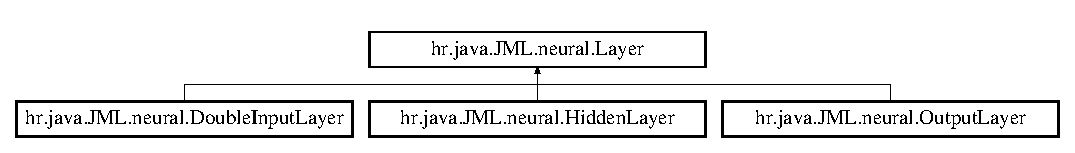
\includegraphics[height=1.602289cm]{classhr_1_1java_1_1_j_m_l_1_1neural_1_1_layer}
\end{center}
\end{figure}
\subsection*{Public Member Functions}
\begin{DoxyCompactItemize}
\item 
\hypertarget{classhr_1_1java_1_1_j_m_l_1_1neural_1_1_layer_ae470877e735c0b6bfd5a6d8b1bf3fcc9}{Double\+Matrix {\bfseries get\+Weights} ()}\label{classhr_1_1java_1_1_j_m_l_1_1neural_1_1_layer_ae470877e735c0b6bfd5a6d8b1bf3fcc9}

\item 
\hypertarget{classhr_1_1java_1_1_j_m_l_1_1neural_1_1_layer_a1bf91d8706c06b60d8d1203e987789eb}{void {\bfseries set\+Weights} (Double\+Matrix weights)}\label{classhr_1_1java_1_1_j_m_l_1_1neural_1_1_layer_a1bf91d8706c06b60d8d1203e987789eb}

\item 
\hypertarget{classhr_1_1java_1_1_j_m_l_1_1neural_1_1_layer_a4d7bb35c7f199394e78505be25776921}{void {\bfseries set\+Num\+Of\+Neurons} (int num\+Of\+Neurons)}\label{classhr_1_1java_1_1_j_m_l_1_1neural_1_1_layer_a4d7bb35c7f199394e78505be25776921}

\item 
\hypertarget{classhr_1_1java_1_1_j_m_l_1_1neural_1_1_layer_a2a4aa1798db11a68b53c794fc929dc25}{\hyperlink{classhr_1_1java_1_1_j_m_l_1_1neural_1_1_layer}{Layer} {\bfseries get\+Previous\+Layer} ()}\label{classhr_1_1java_1_1_j_m_l_1_1neural_1_1_layer_a2a4aa1798db11a68b53c794fc929dc25}

\item 
\hypertarget{classhr_1_1java_1_1_j_m_l_1_1neural_1_1_layer_a92c6d1c7f94f8c99e66413ed40e74685}{void {\bfseries set\+Previous\+Layer} (\hyperlink{classhr_1_1java_1_1_j_m_l_1_1neural_1_1_layer}{Layer} previous\+Layer)}\label{classhr_1_1java_1_1_j_m_l_1_1neural_1_1_layer_a92c6d1c7f94f8c99e66413ed40e74685}

\item 
\hypertarget{classhr_1_1java_1_1_j_m_l_1_1neural_1_1_layer_a2886a423c2f26b7b197ecac8dd2dcefb}{abstract Double\+Vector {\bfseries calculate\+Output} (Double\+Vector input)}\label{classhr_1_1java_1_1_j_m_l_1_1neural_1_1_layer_a2886a423c2f26b7b197ecac8dd2dcefb}

\end{DoxyCompactItemize}
\subsection*{Protected Member Functions}
\begin{DoxyCompactItemize}
\item 
\hypertarget{classhr_1_1java_1_1_j_m_l_1_1neural_1_1_layer_af1af131c8ce496ee145fe366a816ea07}{int {\bfseries get\+Num\+Of\+Neurons} ()}\label{classhr_1_1java_1_1_j_m_l_1_1neural_1_1_layer_af1af131c8ce496ee145fe366a816ea07}

\end{DoxyCompactItemize}
\subsection*{Protected Attributes}
\begin{DoxyCompactItemize}
\item 
\hypertarget{classhr_1_1java_1_1_j_m_l_1_1neural_1_1_layer_a60ed2080e6620f42f632a14e2a8be5aa}{int {\bfseries num\+Of\+Neurons}}\label{classhr_1_1java_1_1_j_m_l_1_1neural_1_1_layer_a60ed2080e6620f42f632a14e2a8be5aa}

\item 
\hypertarget{classhr_1_1java_1_1_j_m_l_1_1neural_1_1_layer_ac6e584a64d1005ca3bf2284da926963e}{Double\+Matrix {\bfseries weights}}\label{classhr_1_1java_1_1_j_m_l_1_1neural_1_1_layer_ac6e584a64d1005ca3bf2284da926963e}

\item 
\hypertarget{classhr_1_1java_1_1_j_m_l_1_1neural_1_1_layer_a236aed43fa2b00808947171931c3b323}{\hyperlink{classhr_1_1java_1_1_j_m_l_1_1neural_1_1_layer}{Layer} {\bfseries previous\+Layer}}\label{classhr_1_1java_1_1_j_m_l_1_1neural_1_1_layer_a236aed43fa2b00808947171931c3b323}

\end{DoxyCompactItemize}


The documentation for this class was generated from the following file\+:\begin{DoxyCompactItemize}
\item 
src/hr/java/\+J\+M\+L/neural/Layer.\+java\end{DoxyCompactItemize}

\hypertarget{classhr_1_1java_1_1_j_m_l_1_1regression_1_1_linear_regression}{\section{hr.\+java.\+J\+M\+L.\+regression.\+Linear\+Regression Class Reference}
\label{classhr_1_1java_1_1_j_m_l_1_1regression_1_1_linear_regression}\index{hr.\+java.\+J\+M\+L.\+regression.\+Linear\+Regression@{hr.\+java.\+J\+M\+L.\+regression.\+Linear\+Regression}}
}
\subsection*{Public Member Functions}
\begin{DoxyCompactItemize}
\item 
\hypertarget{classhr_1_1java_1_1_j_m_l_1_1regression_1_1_linear_regression_a3a0184c391acc975b4c94a72e9c37935}{{\bfseries Linear\+Regression} (double\mbox{[}$\,$\mbox{]}\mbox{[}$\,$\mbox{]} training\+Set, double\mbox{[}$\,$\mbox{]}\mbox{[}$\,$\mbox{]} validation\+Set, double\mbox{[}$\,$\mbox{]}\mbox{[}$\,$\mbox{]} test\+Set, double\mbox{[}$\,$\mbox{]} theta, \hyperlink{classhr_1_1java_1_1_j_m_l_1_1learning_1_1_abstract_minimizer}{Abstract\+Minimizer} minimizer)}\label{classhr_1_1java_1_1_j_m_l_1_1regression_1_1_linear_regression_a3a0184c391acc975b4c94a72e9c37935}

\item 
\hypertarget{classhr_1_1java_1_1_j_m_l_1_1regression_1_1_linear_regression_a39b44929e6d47ff2c3486cead41f6cd3}{{\bfseries Linear\+Regression} (double\mbox{[}$\,$\mbox{]}\mbox{[}$\,$\mbox{]} training\+Set, double\mbox{[}$\,$\mbox{]}\mbox{[}$\,$\mbox{]} validation\+Set, double\mbox{[}$\,$\mbox{]}\mbox{[}$\,$\mbox{]} test\+Set, \hyperlink{classhr_1_1java_1_1_j_m_l_1_1learning_1_1_abstract_minimizer}{Abstract\+Minimizer} minimizer)}\label{classhr_1_1java_1_1_j_m_l_1_1regression_1_1_linear_regression_a39b44929e6d47ff2c3486cead41f6cd3}

\item 
\hypertarget{classhr_1_1java_1_1_j_m_l_1_1regression_1_1_linear_regression_afd01741d15e9a5f7292b410e34add189}{void {\bfseries error\+Limited\+Training} (double desired\+Error)}\label{classhr_1_1java_1_1_j_m_l_1_1regression_1_1_linear_regression_afd01741d15e9a5f7292b410e34add189}

\item 
\hypertarget{classhr_1_1java_1_1_j_m_l_1_1regression_1_1_linear_regression_a8b9f83ea1e115495377fffad26e95577}{void {\bfseries iteration\+Limited\+Training} (int iterations)}\label{classhr_1_1java_1_1_j_m_l_1_1regression_1_1_linear_regression_a8b9f83ea1e115495377fffad26e95577}

\item 
\hypertarget{classhr_1_1java_1_1_j_m_l_1_1regression_1_1_linear_regression_ad35d73add6c9c2e2c7c9e871ed5a391d}{double {\bfseries calculate\+Error} (Double\+Matrix test\+Set, Double\+Vector test\+Set\+Known)}\label{classhr_1_1java_1_1_j_m_l_1_1regression_1_1_linear_regression_ad35d73add6c9c2e2c7c9e871ed5a391d}

\item 
\hypertarget{classhr_1_1java_1_1_j_m_l_1_1regression_1_1_linear_regression_a64031e5cefc57c223b6db2ee49c29698}{void {\bfseries validate\+Training} ()}\label{classhr_1_1java_1_1_j_m_l_1_1regression_1_1_linear_regression_a64031e5cefc57c223b6db2ee49c29698}

\end{DoxyCompactItemize}


The documentation for this class was generated from the following file\+:\begin{DoxyCompactItemize}
\item 
src/hr/java/\+J\+M\+L/regression/Linear\+Regression.\+java\end{DoxyCompactItemize}

\hypertarget{classjava_1_1_j_m_l_1_1test_1_1_linear_regression_test}{\section{java.\+J\+M\+L.\+test.\+Linear\+Regression\+Test Class Reference}
\label{classjava_1_1_j_m_l_1_1test_1_1_linear_regression_test}\index{java.\+J\+M\+L.\+test.\+Linear\+Regression\+Test@{java.\+J\+M\+L.\+test.\+Linear\+Regression\+Test}}
}
\subsection*{Static Public Member Functions}
\begin{DoxyCompactItemize}
\item 
\hypertarget{classjava_1_1_j_m_l_1_1test_1_1_linear_regression_test_a883172d502741a937ceb914080558d5f}{static void {\bfseries main} (String\mbox{[}$\,$\mbox{]} args)}\label{classjava_1_1_j_m_l_1_1test_1_1_linear_regression_test_a883172d502741a937ceb914080558d5f}

\end{DoxyCompactItemize}


The documentation for this class was generated from the following file\+:\begin{DoxyCompactItemize}
\item 
src/java/\+J\+M\+L/test/Linear\+Regression\+Test.\+java\end{DoxyCompactItemize}

\hypertarget{classhr_1_1java_1_1_j_m_l_1_1regression_1_1_logistic_regression}{\section{hr.\+java.\+J\+M\+L.\+regression.\+Logistic\+Regression Class Reference}
\label{classhr_1_1java_1_1_j_m_l_1_1regression_1_1_logistic_regression}\index{hr.\+java.\+J\+M\+L.\+regression.\+Logistic\+Regression@{hr.\+java.\+J\+M\+L.\+regression.\+Logistic\+Regression}}
}
\subsection*{Public Member Functions}
\begin{DoxyCompactItemize}
\item 
\hypertarget{classhr_1_1java_1_1_j_m_l_1_1regression_1_1_logistic_regression_a29f051a57e0a4036fc419b5259ea6104}{{\bfseries Logistic\+Regression} (double\mbox{[}$\,$\mbox{]}\mbox{[}$\,$\mbox{]} training\+Set, double\mbox{[}$\,$\mbox{]}\mbox{[}$\,$\mbox{]} test\+Set, double\mbox{[}$\,$\mbox{]} theta, \hyperlink{classhr_1_1java_1_1_j_m_l_1_1learning_1_1_abstract_minimizer}{Abstract\+Minimizer} minimizer)}\label{classhr_1_1java_1_1_j_m_l_1_1regression_1_1_logistic_regression_a29f051a57e0a4036fc419b5259ea6104}

\item 
\hypertarget{classhr_1_1java_1_1_j_m_l_1_1regression_1_1_logistic_regression_a76653101d8e522d5d4c62094f64461b4}{{\bfseries Logistic\+Regression} (double\mbox{[}$\,$\mbox{]}\mbox{[}$\,$\mbox{]} training\+Set, double\mbox{[}$\,$\mbox{]}\mbox{[}$\,$\mbox{]} test\+Set, \hyperlink{classhr_1_1java_1_1_j_m_l_1_1learning_1_1_abstract_minimizer}{Abstract\+Minimizer} minimizer)}\label{classhr_1_1java_1_1_j_m_l_1_1regression_1_1_logistic_regression_a76653101d8e522d5d4c62094f64461b4}

\item 
\hypertarget{classhr_1_1java_1_1_j_m_l_1_1regression_1_1_logistic_regression_a70e6206c71b5e1a0061e950c72bf31d1}{void {\bfseries error\+Limited\+Training} (double desired\+Error)}\label{classhr_1_1java_1_1_j_m_l_1_1regression_1_1_logistic_regression_a70e6206c71b5e1a0061e950c72bf31d1}

\item 
\hypertarget{classhr_1_1java_1_1_j_m_l_1_1regression_1_1_logistic_regression_a670489f1591d5ea02aba64abf2cd0b0d}{void {\bfseries iteration\+Limited\+Training} (int iterations)}\label{classhr_1_1java_1_1_j_m_l_1_1regression_1_1_logistic_regression_a670489f1591d5ea02aba64abf2cd0b0d}

\item 
\hypertarget{classhr_1_1java_1_1_j_m_l_1_1regression_1_1_logistic_regression_a8b5552490cefdd032f9d0a4baeb87051}{boolean {\bfseries predict} (double\mbox{[}$\,$\mbox{]} features)}\label{classhr_1_1java_1_1_j_m_l_1_1regression_1_1_logistic_regression_a8b5552490cefdd032f9d0a4baeb87051}

\end{DoxyCompactItemize}


The documentation for this class was generated from the following file\+:\begin{DoxyCompactItemize}
\item 
src/hr/java/\+J\+M\+L/regression/Logistic\+Regression.\+java\end{DoxyCompactItemize}

\hypertarget{interfacehr_1_1java_1_1_j_m_l_1_1learning_1_1_minimizer}{\section{hr.\+java.\+J\+M\+L.\+learning.\+Minimizer Interface Reference}
\label{interfacehr_1_1java_1_1_j_m_l_1_1learning_1_1_minimizer}\index{hr.\+java.\+J\+M\+L.\+learning.\+Minimizer@{hr.\+java.\+J\+M\+L.\+learning.\+Minimizer}}
}
Inheritance diagram for hr.\+java.\+J\+M\+L.\+learning.\+Minimizer\+:\begin{figure}[H]
\begin{center}
\leavevmode
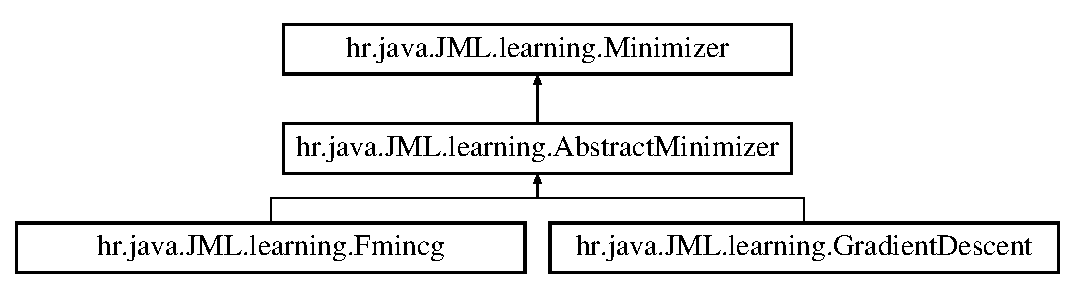
\includegraphics[height=3.000000cm]{interfacehr_1_1java_1_1_j_m_l_1_1learning_1_1_minimizer}
\end{center}
\end{figure}
\subsection*{Public Member Functions}
\begin{DoxyCompactItemize}
\item 
Double\+Vector \hyperlink{interfacehr_1_1java_1_1_j_m_l_1_1learning_1_1_minimizer_a4b640a5d2cc5293ccc47736a798c6ab7}{minimize} (\hyperlink{interfacehr_1_1java_1_1_j_m_l_1_1cost_1_1_cost_function}{Cost\+Function} f, Double\+Vector theta, int max\+Iterations, boolean verbose)
\end{DoxyCompactItemize}


\subsection{Detailed Description}
\hyperlink{interfacehr_1_1java_1_1_j_m_l_1_1learning_1_1_minimizer}{Minimizer} interface for various function minimizers.

\begin{DoxyAuthor}{Author}
thomas.\+jungblut 
\end{DoxyAuthor}


\subsection{Member Function Documentation}
\hypertarget{interfacehr_1_1java_1_1_j_m_l_1_1learning_1_1_minimizer_a4b640a5d2cc5293ccc47736a798c6ab7}{\index{hr\+::java\+::\+J\+M\+L\+::learning\+::\+Minimizer@{hr\+::java\+::\+J\+M\+L\+::learning\+::\+Minimizer}!minimize@{minimize}}
\index{minimize@{minimize}!hr\+::java\+::\+J\+M\+L\+::learning\+::\+Minimizer@{hr\+::java\+::\+J\+M\+L\+::learning\+::\+Minimizer}}
\subsubsection[{minimize}]{\setlength{\rightskip}{0pt plus 5cm}Double\+Vector hr.\+java.\+J\+M\+L.\+learning.\+Minimizer.\+minimize (
\begin{DoxyParamCaption}
\item[{{\bf Cost\+Function}}]{f, }
\item[{Double\+Vector}]{theta, }
\item[{int}]{max\+Iterations, }
\item[{boolean}]{verbose}
\end{DoxyParamCaption}
)}}\label{interfacehr_1_1java_1_1_j_m_l_1_1learning_1_1_minimizer_a4b640a5d2cc5293ccc47736a798c6ab7}
Minimizes the given costfunction with the starting parameter theta.


\begin{DoxyParams}{Parameters}
{\em f} & the costfunction to minimize. \\
\hline
{\em theta} & the starting parameters. \\
\hline
{\em max\+Iterations} & the number of iterations to do. \\
\hline
{\em verbose} & if T\+R\+U\+E it will print progress. \\
\hline
\end{DoxyParams}
\begin{DoxyReturn}{Returns}
the optimized theta parameters. 
\end{DoxyReturn}


Implemented in \hyperlink{classhr_1_1java_1_1_j_m_l_1_1learning_1_1_fmincg_a91e1dfdbc2222e1844a3c6d079a7e3e7}{hr.\+java.\+J\+M\+L.\+learning.\+Fmincg}.



The documentation for this interface was generated from the following file\+:\begin{DoxyCompactItemize}
\item 
src/hr/java/\+J\+M\+L/learning/Minimizer.\+java\end{DoxyCompactItemize}

\hypertarget{interfacehr_1_1java_1_1_j_m_l_1_1neural_1_1_neural_cost_function}{\section{hr.\+java.\+J\+M\+L.\+neural.\+Neural\+Cost\+Function Interface Reference}
\label{interfacehr_1_1java_1_1_j_m_l_1_1neural_1_1_neural_cost_function}\index{hr.\+java.\+J\+M\+L.\+neural.\+Neural\+Cost\+Function@{hr.\+java.\+J\+M\+L.\+neural.\+Neural\+Cost\+Function}}
}
\subsection*{Public Member Functions}
\begin{DoxyCompactItemize}
\item 
\hyperlink{classhr_1_1java_1_1_j_m_l_1_1neural_1_1_neural_cost_gradient_tuple}{Neural\+Cost\+Gradient\+Tuple} \hyperlink{interfacehr_1_1java_1_1_j_m_l_1_1neural_1_1_neural_cost_function_addee0abd0a0bf0505b1e697b57467224}{evaluate\+Cost} (Double\+Matrix input, Double\+Vector expected)
\end{DoxyCompactItemize}


\subsection{Detailed Description}
Cost function interface to be implemented when using with a optimizer like conjugate gradient for example.

\begin{DoxyAuthor}{Author}
thomas.\+jungblut 
\end{DoxyAuthor}


\subsection{Member Function Documentation}
\hypertarget{interfacehr_1_1java_1_1_j_m_l_1_1neural_1_1_neural_cost_function_addee0abd0a0bf0505b1e697b57467224}{\index{hr\+::java\+::\+J\+M\+L\+::neural\+::\+Neural\+Cost\+Function@{hr\+::java\+::\+J\+M\+L\+::neural\+::\+Neural\+Cost\+Function}!evaluate\+Cost@{evaluate\+Cost}}
\index{evaluate\+Cost@{evaluate\+Cost}!hr\+::java\+::\+J\+M\+L\+::neural\+::\+Neural\+Cost\+Function@{hr\+::java\+::\+J\+M\+L\+::neural\+::\+Neural\+Cost\+Function}}
\subsubsection[{evaluate\+Cost}]{\setlength{\rightskip}{0pt plus 5cm}{\bf Neural\+Cost\+Gradient\+Tuple} hr.\+java.\+J\+M\+L.\+neural.\+Neural\+Cost\+Function.\+evaluate\+Cost (
\begin{DoxyParamCaption}
\item[{Double\+Matrix}]{input, }
\item[{Double\+Vector}]{expected}
\end{DoxyParamCaption}
)}}\label{interfacehr_1_1java_1_1_j_m_l_1_1neural_1_1_neural_cost_function_addee0abd0a0bf0505b1e697b57467224}
Evaluation for the cost function to retrieve cost and gradient.


\begin{DoxyParams}{Parameters}
{\em input} & a given input vector \\
\hline
\end{DoxyParams}
\begin{DoxyReturn}{Returns}
a tuple consists of J (cost) and a vector X which is the gradient of the input. 
\end{DoxyReturn}


The documentation for this interface was generated from the following file\+:\begin{DoxyCompactItemize}
\item 
src/hr/java/\+J\+M\+L/neural/Neural\+Cost\+Function.\+java\end{DoxyCompactItemize}

\hypertarget{classhr_1_1java_1_1_j_m_l_1_1neural_1_1_neural_cost_gradient_tuple}{\section{hr.\+java.\+J\+M\+L.\+neural.\+Neural\+Cost\+Gradient\+Tuple Class Reference}
\label{classhr_1_1java_1_1_j_m_l_1_1neural_1_1_neural_cost_gradient_tuple}\index{hr.\+java.\+J\+M\+L.\+neural.\+Neural\+Cost\+Gradient\+Tuple@{hr.\+java.\+J\+M\+L.\+neural.\+Neural\+Cost\+Gradient\+Tuple}}
}
\subsection*{Public Member Functions}
\begin{DoxyCompactItemize}
\item 
\hypertarget{classhr_1_1java_1_1_j_m_l_1_1neural_1_1_neural_cost_gradient_tuple_a46fe2e7f1fb0c65b3c9f5e56e49f31e3}{{\bfseries Neural\+Cost\+Gradient\+Tuple} (double cost, Double\+Vector gradient)}\label{classhr_1_1java_1_1_j_m_l_1_1neural_1_1_neural_cost_gradient_tuple_a46fe2e7f1fb0c65b3c9f5e56e49f31e3}

\item 
\hypertarget{classhr_1_1java_1_1_j_m_l_1_1neural_1_1_neural_cost_gradient_tuple_ac0b348d079d3d3bb121501a3198a5e2a}{double {\bfseries get\+Cost} ()}\label{classhr_1_1java_1_1_j_m_l_1_1neural_1_1_neural_cost_gradient_tuple_ac0b348d079d3d3bb121501a3198a5e2a}

\item 
\hypertarget{classhr_1_1java_1_1_j_m_l_1_1neural_1_1_neural_cost_gradient_tuple_afe8955a29eeae12780025db1c94ac4c9}{Double\+Vector {\bfseries get\+Gradient} ()}\label{classhr_1_1java_1_1_j_m_l_1_1neural_1_1_neural_cost_gradient_tuple_afe8955a29eeae12780025db1c94ac4c9}

\end{DoxyCompactItemize}


\subsection{Detailed Description}
More readable variant of the before used Tuple$<$$>$ in \hyperlink{}{Cost\+Function}.

\begin{DoxyAuthor}{Author}
thomas.\+jungblut 
\end{DoxyAuthor}


The documentation for this class was generated from the following file\+:\begin{DoxyCompactItemize}
\item 
src/hr/java/\+J\+M\+L/neural/Neural\+Cost\+Gradient\+Tuple.\+java\end{DoxyCompactItemize}

\hypertarget{classhr_1_1java_1_1_j_m_l_1_1neural_1_1_neural_network}{\section{hr.\+java.\+J\+M\+L.\+neural.\+Neural\+Network Class Reference}
\label{classhr_1_1java_1_1_j_m_l_1_1neural_1_1_neural_network}\index{hr.\+java.\+J\+M\+L.\+neural.\+Neural\+Network@{hr.\+java.\+J\+M\+L.\+neural.\+Neural\+Network}}
}
\subsection*{Public Member Functions}
\begin{DoxyCompactItemize}
\item 
\hypertarget{classhr_1_1java_1_1_j_m_l_1_1neural_1_1_neural_network_a4c7d73c9236cc35114a2f1dda0eb2ca7}{{\bfseries Neural\+Network} (double\mbox{[}$\,$\mbox{]}\mbox{[}$\,$\mbox{]} training\+Set, double\mbox{[}$\,$\mbox{]}\mbox{[}$\,$\mbox{]} test\+Set, int num\+Of\+Labels, int num\+Of\+Hidden, int\mbox{[}$\,$\mbox{]} size\+Of\+Hidden, \hyperlink{classhr_1_1java_1_1_j_m_l_1_1activation_functions_1_1_activation_function}{Activation\+Function} af, \hyperlink{classhr_1_1java_1_1_j_m_l_1_1learning_1_1_abstract_minimizer}{Abstract\+Minimizer} minimizer)}\label{classhr_1_1java_1_1_j_m_l_1_1neural_1_1_neural_network_a4c7d73c9236cc35114a2f1dda0eb2ca7}

\item 
\hypertarget{classhr_1_1java_1_1_j_m_l_1_1neural_1_1_neural_network_a3d05b487280ce8d3f4b51422a47e012c}{void {\bfseries train\+Till\+Error} (double desired\+Error)}\label{classhr_1_1java_1_1_j_m_l_1_1neural_1_1_neural_network_a3d05b487280ce8d3f4b51422a47e012c}

\item 
\hypertarget{classhr_1_1java_1_1_j_m_l_1_1neural_1_1_neural_network_a59b297e03c2eb941d21abcee66a9723f}{void {\bfseries iteration\+Limited\+Training} (int iterations)}\label{classhr_1_1java_1_1_j_m_l_1_1neural_1_1_neural_network_a59b297e03c2eb941d21abcee66a9723f}

\item 
\hypertarget{classhr_1_1java_1_1_j_m_l_1_1neural_1_1_neural_network_a5e34cbf0f22a97389d219344a2d96f61}{Double\+Vector {\bfseries get\+Folded\+Theta\+Vector} ()}\label{classhr_1_1java_1_1_j_m_l_1_1neural_1_1_neural_network_a5e34cbf0f22a97389d219344a2d96f61}

\item 
\hypertarget{classhr_1_1java_1_1_j_m_l_1_1neural_1_1_neural_network_a46ce5f1a17a3c3d0cd92fb1c985b5d47}{int\mbox{[}$\,$\mbox{]}\mbox{[}$\,$\mbox{]} {\bfseries compute\+Unfold\+Parameters} ()}\label{classhr_1_1java_1_1_j_m_l_1_1neural_1_1_neural_network_a46ce5f1a17a3c3d0cd92fb1c985b5d47}

\end{DoxyCompactItemize}
\subsection*{Protected Attributes}
\begin{DoxyCompactItemize}
\item 
\hypertarget{classhr_1_1java_1_1_j_m_l_1_1neural_1_1_neural_network_a522ff13cc9fa9d4ab160032a0bf182f9}{int\mbox{[}$\,$\mbox{]}\mbox{[}$\,$\mbox{]} {\bfseries size\+Array}}\label{classhr_1_1java_1_1_j_m_l_1_1neural_1_1_neural_network_a522ff13cc9fa9d4ab160032a0bf182f9}

\end{DoxyCompactItemize}
\subsection*{Static Protected Attributes}
\begin{DoxyCompactItemize}
\item 
\hypertarget{classhr_1_1java_1_1_j_m_l_1_1neural_1_1_neural_network_a40416a35caa49558ee5d030d1f77de69}{static final double {\bfseries L\+A\+M\+B\+D\+A} = 0.\+5}\label{classhr_1_1java_1_1_j_m_l_1_1neural_1_1_neural_network_a40416a35caa49558ee5d030d1f77de69}

\end{DoxyCompactItemize}


The documentation for this class was generated from the following file\+:\begin{DoxyCompactItemize}
\item 
src/hr/java/\+J\+M\+L/neural/Neural\+Network.\+java\end{DoxyCompactItemize}

\hypertarget{classhr_1_1java_1_1_j_m_l_1_1exceptions_1_1_not_trained_exception}{\section{hr.\+java.\+J\+M\+L.\+exceptions.\+Not\+Trained\+Exception Class Reference}
\label{classhr_1_1java_1_1_j_m_l_1_1exceptions_1_1_not_trained_exception}\index{hr.\+java.\+J\+M\+L.\+exceptions.\+Not\+Trained\+Exception@{hr.\+java.\+J\+M\+L.\+exceptions.\+Not\+Trained\+Exception}}
}
Inheritance diagram for hr.\+java.\+J\+M\+L.\+exceptions.\+Not\+Trained\+Exception\+:\begin{figure}[H]
\begin{center}
\leavevmode
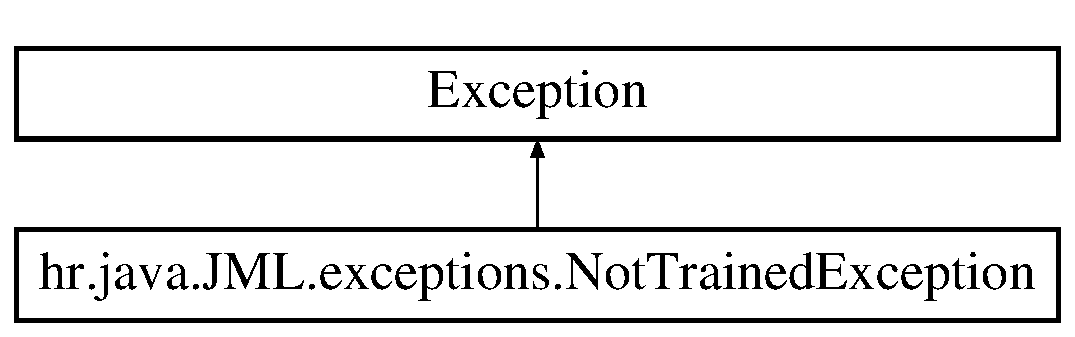
\includegraphics[height=2.000000cm]{classhr_1_1java_1_1_j_m_l_1_1exceptions_1_1_not_trained_exception}
\end{center}
\end{figure}
\subsection*{Public Member Functions}
\begin{DoxyCompactItemize}
\item 
\hypertarget{classhr_1_1java_1_1_j_m_l_1_1exceptions_1_1_not_trained_exception_a9172476b070bad6b53d178cb90c2779b}{{\bfseries Not\+Trained\+Exception} (String message)}\label{classhr_1_1java_1_1_j_m_l_1_1exceptions_1_1_not_trained_exception_a9172476b070bad6b53d178cb90c2779b}

\item 
\hypertarget{classhr_1_1java_1_1_j_m_l_1_1exceptions_1_1_not_trained_exception_a313bc1885ad94faaef5c1af2f42fe4b0}{{\bfseries Not\+Trained\+Exception} (Throwable cause)}\label{classhr_1_1java_1_1_j_m_l_1_1exceptions_1_1_not_trained_exception_a313bc1885ad94faaef5c1af2f42fe4b0}

\item 
\hypertarget{classhr_1_1java_1_1_j_m_l_1_1exceptions_1_1_not_trained_exception_afa8cb67117d7fd01887284362103a302}{{\bfseries Not\+Trained\+Exception} (String message, Throwable cause)}\label{classhr_1_1java_1_1_j_m_l_1_1exceptions_1_1_not_trained_exception_afa8cb67117d7fd01887284362103a302}

\item 
\hypertarget{classhr_1_1java_1_1_j_m_l_1_1exceptions_1_1_not_trained_exception_a5ecdd38a7209e31688c83407517ada73}{{\bfseries Not\+Trained\+Exception} (String message, Throwable cause, boolean enable\+Suppression, boolean writable\+Stack\+Trace)}\label{classhr_1_1java_1_1_j_m_l_1_1exceptions_1_1_not_trained_exception_a5ecdd38a7209e31688c83407517ada73}

\end{DoxyCompactItemize}


The documentation for this class was generated from the following file\+:\begin{DoxyCompactItemize}
\item 
src/hr/java/\+J\+M\+L/exceptions/Not\+Trained\+Exception.\+java\end{DoxyCompactItemize}

\hypertarget{classhr_1_1java_1_1_j_m_l_1_1regression_1_1_one_versus_all}{\section{hr.\+java.\+J\+M\+L.\+regression.\+One\+Versus\+All Class Reference}
\label{classhr_1_1java_1_1_j_m_l_1_1regression_1_1_one_versus_all}\index{hr.\+java.\+J\+M\+L.\+regression.\+One\+Versus\+All@{hr.\+java.\+J\+M\+L.\+regression.\+One\+Versus\+All}}
}
\subsection*{Public Member Functions}
\begin{DoxyCompactItemize}
\item 
\hypertarget{classhr_1_1java_1_1_j_m_l_1_1regression_1_1_one_versus_all_a40915e7a024e823e81488fe648ff8b7d}{{\bfseries One\+Versus\+All} (double\mbox{[}$\,$\mbox{]}\mbox{[}$\,$\mbox{]} training\+Set, double\mbox{[}$\,$\mbox{]}\mbox{[}$\,$\mbox{]} test\+Set, double\mbox{[}$\,$\mbox{]}\mbox{[}$\,$\mbox{]} theta, int\mbox{[}$\,$\mbox{]} classifiers, \hyperlink{classhr_1_1java_1_1_j_m_l_1_1learning_1_1_abstract_minimizer}{Abstract\+Minimizer} minimizer)}\label{classhr_1_1java_1_1_j_m_l_1_1regression_1_1_one_versus_all_a40915e7a024e823e81488fe648ff8b7d}

\item 
\hypertarget{classhr_1_1java_1_1_j_m_l_1_1regression_1_1_one_versus_all_a5ab53916e2a41e3a8e2c81d359beb837}{{\bfseries One\+Versus\+All} (double\mbox{[}$\,$\mbox{]}\mbox{[}$\,$\mbox{]} training\+Set, double\mbox{[}$\,$\mbox{]}\mbox{[}$\,$\mbox{]} test\+Set, Array\+List$<$ String $>$ classifiers, \hyperlink{classhr_1_1java_1_1_j_m_l_1_1learning_1_1_abstract_minimizer}{Abstract\+Minimizer} minimizer)}\label{classhr_1_1java_1_1_j_m_l_1_1regression_1_1_one_versus_all_a5ab53916e2a41e3a8e2c81d359beb837}

\item 
\hypertarget{classhr_1_1java_1_1_j_m_l_1_1regression_1_1_one_versus_all_a9df5980a7439bd6af0792ed8315c9d90}{void {\bfseries error\+Limited\+Training} (double desired\+Error)}\label{classhr_1_1java_1_1_j_m_l_1_1regression_1_1_one_versus_all_a9df5980a7439bd6af0792ed8315c9d90}

\item 
\hypertarget{classhr_1_1java_1_1_j_m_l_1_1regression_1_1_one_versus_all_a447ae53e368ae6125531f6fb35d5ad62}{void {\bfseries iteration\+Limited\+Training} (int iterations)}\label{classhr_1_1java_1_1_j_m_l_1_1regression_1_1_one_versus_all_a447ae53e368ae6125531f6fb35d5ad62}

\item 
\hypertarget{classhr_1_1java_1_1_j_m_l_1_1regression_1_1_one_versus_all_ac87907964da0bf8b9b190325f5f4be26}{Double\+Vector {\bfseries predict} (Double\+Matrix set)}\label{classhr_1_1java_1_1_j_m_l_1_1regression_1_1_one_versus_all_ac87907964da0bf8b9b190325f5f4be26}

\end{DoxyCompactItemize}


The documentation for this class was generated from the following file\+:\begin{DoxyCompactItemize}
\item 
src/hr/java/\+J\+M\+L/regression/One\+Versus\+All.\+java\end{DoxyCompactItemize}

\hypertarget{classhr_1_1java_1_1_j_m_l_1_1neural_1_1_output_layer}{\section{hr.\+java.\+J\+M\+L.\+neural.\+Output\+Layer Class Reference}
\label{classhr_1_1java_1_1_j_m_l_1_1neural_1_1_output_layer}\index{hr.\+java.\+J\+M\+L.\+neural.\+Output\+Layer@{hr.\+java.\+J\+M\+L.\+neural.\+Output\+Layer}}
}
Inheritance diagram for hr.\+java.\+J\+M\+L.\+neural.\+Output\+Layer\+:\begin{figure}[H]
\begin{center}
\leavevmode
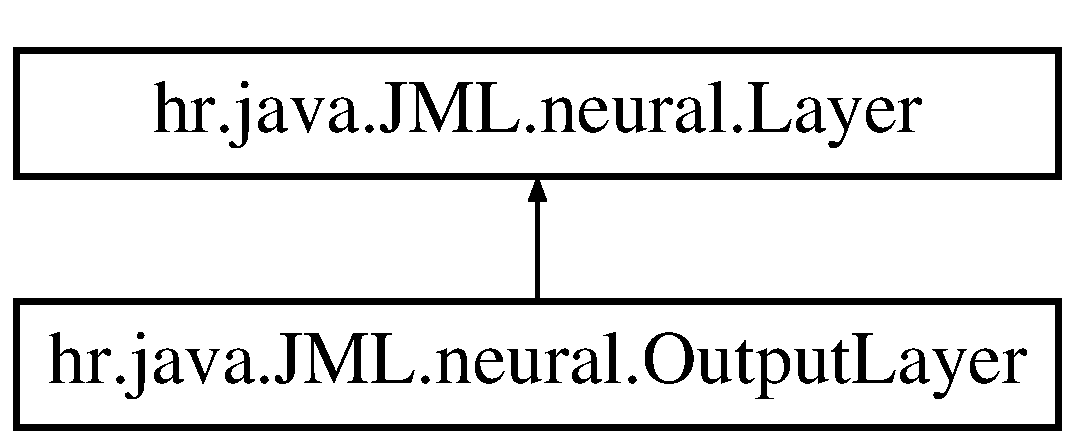
\includegraphics[height=2.000000cm]{classhr_1_1java_1_1_j_m_l_1_1neural_1_1_output_layer}
\end{center}
\end{figure}
\subsection*{Public Member Functions}
\begin{DoxyCompactItemize}
\item 
\hypertarget{classhr_1_1java_1_1_j_m_l_1_1neural_1_1_output_layer_a60cd948faf2fe4049151502c42a875b5}{{\bfseries Output\+Layer} (int size, \hyperlink{classhr_1_1java_1_1_j_m_l_1_1neural_1_1_layer}{Layer} prev, \hyperlink{classhr_1_1java_1_1_j_m_l_1_1activation_functions_1_1_activation_function}{Activation\+Function} af)}\label{classhr_1_1java_1_1_j_m_l_1_1neural_1_1_output_layer_a60cd948faf2fe4049151502c42a875b5}

\item 
\hypertarget{classhr_1_1java_1_1_j_m_l_1_1neural_1_1_output_layer_a5847f429677ba90474f98106eefc3a04}{Double\+Matrix {\bfseries get\+Weights} ()}\label{classhr_1_1java_1_1_j_m_l_1_1neural_1_1_output_layer_a5847f429677ba90474f98106eefc3a04}

\item 
\hypertarget{classhr_1_1java_1_1_j_m_l_1_1neural_1_1_output_layer_a04ec7b94907cdecc318a566e35c51f1b}{void {\bfseries set\+Weights} (Double\+Matrix weights)}\label{classhr_1_1java_1_1_j_m_l_1_1neural_1_1_output_layer_a04ec7b94907cdecc318a566e35c51f1b}

\item 
\hypertarget{classhr_1_1java_1_1_j_m_l_1_1neural_1_1_output_layer_a5b7d4d95e60adc494c27bd3a87901202}{void {\bfseries set\+Weights\+By\+Neuron} (Double\+Matrix weights)}\label{classhr_1_1java_1_1_j_m_l_1_1neural_1_1_output_layer_a5b7d4d95e60adc494c27bd3a87901202}

\item 
\hypertarget{classhr_1_1java_1_1_j_m_l_1_1neural_1_1_output_layer_abe9a367c255585c18beb2901f6bf2c89}{Double\+Vector {\bfseries calculate\+Output} (Double\+Vector input)}\label{classhr_1_1java_1_1_j_m_l_1_1neural_1_1_output_layer_abe9a367c255585c18beb2901f6bf2c89}

\end{DoxyCompactItemize}
\subsection*{Additional Inherited Members}


The documentation for this class was generated from the following file\+:\begin{DoxyCompactItemize}
\item 
src/hr/java/\+J\+M\+L/neural/Output\+Layer.\+java\end{DoxyCompactItemize}

\hypertarget{classhr_1_1java_1_1_j_m_l_1_1activation_functions_1_1_sigmoid_activation_function}{\section{hr.\+java.\+J\+M\+L.\+activation\+Functions.\+Sigmoid\+Activation\+Function Class Reference}
\label{classhr_1_1java_1_1_j_m_l_1_1activation_functions_1_1_sigmoid_activation_function}\index{hr.\+java.\+J\+M\+L.\+activation\+Functions.\+Sigmoid\+Activation\+Function@{hr.\+java.\+J\+M\+L.\+activation\+Functions.\+Sigmoid\+Activation\+Function}}
}
Inheritance diagram for hr.\+java.\+J\+M\+L.\+activation\+Functions.\+Sigmoid\+Activation\+Function\+:\begin{figure}[H]
\begin{center}
\leavevmode
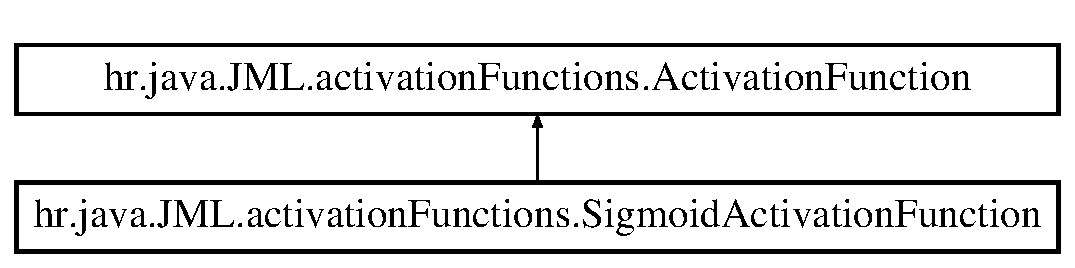
\includegraphics[height=2.000000cm]{classhr_1_1java_1_1_j_m_l_1_1activation_functions_1_1_sigmoid_activation_function}
\end{center}
\end{figure}
\subsection*{Public Member Functions}
\begin{DoxyCompactItemize}
\item 
\hypertarget{classhr_1_1java_1_1_j_m_l_1_1activation_functions_1_1_sigmoid_activation_function_a702f077516bb8f658da835e96f317446}{double {\bfseries activation\+Function} (double input)}\label{classhr_1_1java_1_1_j_m_l_1_1activation_functions_1_1_sigmoid_activation_function_a702f077516bb8f658da835e96f317446}

\item 
\hypertarget{classhr_1_1java_1_1_j_m_l_1_1activation_functions_1_1_sigmoid_activation_function_aaa6e666ecd62804576e5295ddbabca0c}{Double\+Vector {\bfseries activation\+Function} (Double\+Vector input)}\label{classhr_1_1java_1_1_j_m_l_1_1activation_functions_1_1_sigmoid_activation_function_aaa6e666ecd62804576e5295ddbabca0c}

\item 
\hypertarget{classhr_1_1java_1_1_j_m_l_1_1activation_functions_1_1_sigmoid_activation_function_a53a843666b3ee22fe797fbdd36ed0b12}{Double\+Vector {\bfseries gradient} (Double\+Vector input)}\label{classhr_1_1java_1_1_j_m_l_1_1activation_functions_1_1_sigmoid_activation_function_a53a843666b3ee22fe797fbdd36ed0b12}

\item 
\hypertarget{classhr_1_1java_1_1_j_m_l_1_1activation_functions_1_1_sigmoid_activation_function_ad171e4ccf0c2d891a470dd7bbbb7b084}{Double\+Matrix {\bfseries activation\+Function} (Double\+Matrix input)}\label{classhr_1_1java_1_1_j_m_l_1_1activation_functions_1_1_sigmoid_activation_function_ad171e4ccf0c2d891a470dd7bbbb7b084}

\item 
\hypertarget{classhr_1_1java_1_1_j_m_l_1_1activation_functions_1_1_sigmoid_activation_function_a4a3fc77fb29697da7e7dd9445360da4d}{Double\+Matrix {\bfseries gradient} (Double\+Matrix input)}\label{classhr_1_1java_1_1_j_m_l_1_1activation_functions_1_1_sigmoid_activation_function_a4a3fc77fb29697da7e7dd9445360da4d}

\end{DoxyCompactItemize}


\subsection{Detailed Description}
\begin{DoxyAuthor}{Author}
Filip Habazin Computes the activation potentials and gradients for the Sigmoid activation function. the sigmoid is described as f(x)=1/(e$^\wedge$-\/x). 
\end{DoxyAuthor}


The documentation for this class was generated from the following file\+:\begin{DoxyCompactItemize}
\item 
src/hr/java/\+J\+M\+L/activation\+Functions/Sigmoid\+Activation\+Function.\+java\end{DoxyCompactItemize}

\hypertarget{classhr_1_1java_1_1_j_m_l_1_1clustering_1_1_vectors_not_equal_length_exception}{\section{hr.\+java.\+J\+M\+L.\+clustering.\+Vectors\+Not\+Equal\+Length\+Exception Class Reference}
\label{classhr_1_1java_1_1_j_m_l_1_1clustering_1_1_vectors_not_equal_length_exception}\index{hr.\+java.\+J\+M\+L.\+clustering.\+Vectors\+Not\+Equal\+Length\+Exception@{hr.\+java.\+J\+M\+L.\+clustering.\+Vectors\+Not\+Equal\+Length\+Exception}}
}
Inheritance diagram for hr.\+java.\+J\+M\+L.\+clustering.\+Vectors\+Not\+Equal\+Length\+Exception\+:\begin{figure}[H]
\begin{center}
\leavevmode
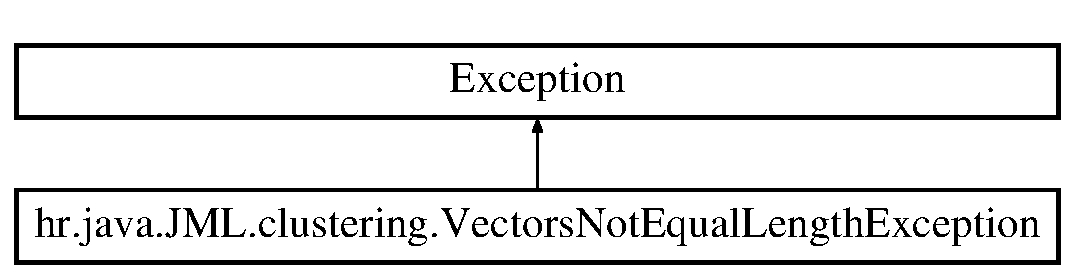
\includegraphics[height=2.000000cm]{classhr_1_1java_1_1_j_m_l_1_1clustering_1_1_vectors_not_equal_length_exception}
\end{center}
\end{figure}


The documentation for this class was generated from the following file\+:\begin{DoxyCompactItemize}
\item 
src/hr/java/\+J\+M\+L/clustering/Vectors\+Not\+Equal\+Length\+Exception.\+java\end{DoxyCompactItemize}

%--- End generated contents ---

% Index
\newpage
\phantomsection
\addcontentsline{toc}{chapter}{Index}
\printindex

\end{document}
